% MDPI Games Research Article -- Overleaf main.tex
% Requires the OFFICIAL MDPI Definitions/ folder in the Overleaf project.
% Import this ZIP into an existing MDPI template project, or copy its
% Definitions folder into this project. No modified mdpi.cls is supplied.
\documentclass[games,article,submit,moreauthors]{Definitions/mdpi}

% MDPI class loads amsmath, amssymb, graphicx, natbib, booktabs,
% tabularx, cleveref, hyperref, and amsthm. Avoid package duplication.
\firstpage{1}
\makeatletter
\setcounter{page}{\@firstpage}
\makeatother
\pubvolume{1}
\issuenum{1}
\articlenumber{0}
\pubyear{2026}
\copyrightyear{2026}
\datereceived{ }
\daterevised{ }
\dateaccepted{ }
\datepublished{ }

\Title{A Game-Theoretic Framework for Competitive Seeding in Conway's Game of Life: Equilibrium Structure, Randomized Baselines, and NES Validation}

\newcommand{\orcidauthorA}{0000-0002-6005-2473} % Add \orcidA{} behind the author's name

% The exact author names and affiliation numbering below follow the provided
% ALife2026 manuscript. ORCIDs and corresponding-author details are pending.
\Author{Bruno Senzio-Savino $^{1}$\orcidA{}, Faramarz Alsharif $^{2}$, Aleksandar Shurbevski $^{3}$ and Mahdi Khosravy $^{3,4}$}
\AuthorNames{Bruno Senzio-Savino, Faramarz Alsharif, Aleksandar Shurbevski and Mahdi Khosravy}
\address{%
$^{1}$ \quad Graduate School of Science and Engineering, Department of Informatics and Electronics, Electrical and Electronics Communication Engineering, Yamagata University, Japan (Invited Researcher)\\
$^{2}$ \quad Graduate School of Science and Engineering, Department of Informatics and Electronics, Electrical and Electronics Communication Engineering, Yamagata University, Japan\\
$^{3}$ \quad The Kyoto College of Graduate Studies for Informatics, Kyoto, Japan\\
$^{4}$ \quad CrossCompass Ltd., Tokyo, Japan}
\corres{Correspondence: asharif@yz.yamagata-u.ac.jp}

\abstract{Competition over a cellular automaton's initial conditions offers a finite strategic interaction without changing its local rules. We formulate a two-player zero-sum seeding game on a finite $5\times5$ Conway Game of Life board. The players select fixed-cardinality, nonoverlapping seed patterns; the row player maximizes and the column player minimizes the number of live cells at the tenth recorded generation. We study pure and mixed equilibria across seed budgets of three to seven cells and restricted action sets of 3, 5, and 10 patterns per player. In 1,500 sampled games, the fraction lacking a pure equilibrium increases from 15\% to 51\% at budget three and from 53\% to 99\% at budget seven when the action count increases from three to ten. A within-matrix permutation baseline, preserving each payoff multiset and its ties, exhibits higher no-pure-equilibrium rates in all 15 examined conditions, with heterogeneous effect sizes. Spatial transformations also alter equilibrium existence. Ten selected computational trajectories were compared with records from an NES implementation, yielding 100 matching board states (2,500 matching cell states). These results characterize restricted Conway-induced games, not the unrestricted automaton, and link the NES platform to computational game theory.}
\keyword{algorithmic game theory; Conway's Game of Life; Nash equilibrium; minimax; competitive seeding; cellular automata; permutation baseline; Nintendo Entertainment System; reproducibility}

\begin{document}

\section{Introduction}\label{sec:introduction}

Conway's Game of Life (GoL) is a deterministic cellular automaton in which local birth and survival rules generate complex temporal behavior from an initial binary configuration \citep{gardner1970,wolfram2002}. Initial configurations are therefore a natural control surface: a small modification to the positions of live cells can alter the trajectory of the entire board. However, choosing an initial configuration becomes a strategic problem only after specifying decision makers, feasible actions, competing objectives, and an outcome-dependent utility function. In particular, the presence of a playable video game does not, by itself, imply the existence of a formal game-theoretic model.

Competitive versions of Life are not unprecedented. The two-player automaton developed by \citet{levene2003} introduces competing cell types and modifies the transition mechanism. Competitive evolutionary studies based on the Immigration Game similarly use distinguishable lineages and a modified competitive interpretation \citep{turney2021}. In a different domain, competitive diffusion games model initial seed choices and investigate the structure and computational complexity of equilibria on networks \citep{etesami2016}. Spatial noncooperative games likewise demonstrate that geometry and the rules of interaction influence equilibrium outcomes \citep{andrade2009}. These precedents establish that neither two-player cellular automata nor competitive seeding is novel in isolation.

Our focus differs in three ways. First, \emph{the standard Conway B3/S23 update rule is kept unchanged}. In this notation, B3 indicates that a dead cell becomes alive when exactly three of its eight neighbors are alive, whereas S23 indicates that a living cell survives when it has two or three living neighbors. All other cells become or remain dead. These rules are applied synchronously and are formally defined in Equation~\eqref{eq:conway}. Competition is imposed entirely through external payoff functions associated with the final population of an otherwise ordinary binary automaton. Second, we study restricted, finite normal-form games generated by spatially separated seed-placement choices, with both pure and mixed Nash equilibria computed explicitly. Third, we test whether their observed equilibrium structure differs from controls constructed by permuting the entries of each empirical payoff matrix while exactly preserving its payoff distribution, including ties.

Artificial-life research has long treated simple local interactions as a route to emergent behavior \citep{langton1989artificial,ilachinski2001cellular}. Historical accounts trace how artificial-life research connected computational models to questions about life-like organization \citep{levy1992}. Evolutionary computing provides a related but distinct family of approaches in which populations of candidate solutions are varied and selected \citep{eiben2015evolutionary}; our experiments do not use an evolutionary optimizer, and Conway states evolve solely through fixed B3/S23 rules. Interactive computational environments can additionally expose the role of user-defined initial conditions \citep{resnick2001turtles}. The computational formulation is motivated by an existing NES/Famicom artificial-life implementation. In that system, a user first collects virtual vegetables, defining a seed budget, and then initializes a $5\times5$ GoL board through manual or random placement. The console subsequently displays the automaton's evolution. The \emph{two-player strategic model is a separate Python-based analytical extension}, not a claim that competitive multiplayer play or Nash-equilibrium computation is implemented in the NES ROM. We use the console implementation as an independent execution environment for selected trajectories.

The research questions are: (RQ1) how frequently do restricted Conway-induced games possess pure-strategy saddle points; (RQ2) how do strategy-set size and spatial arrangement change equilibrium structure; (RQ3) does the row--column organization of the payoff matrices differ from tie-preserving randomized controls; and (RQ4) do selected predicted trajectories agree with the implemented NES evolution? The main contributions are a precise game definition and computational protocol, an empirical equilibrium analysis over several controlled strategy families, a payoff-permutation comparison, and a cell-level NES--Python validation protocol. The present study does not test human decision making or learning.

\section{Materials and Methods}\label{sec:methods}

\subsection{Interactive NES Origin and Scope of the Formal Extension}

The previously developed NES system, documented in the earlier platform paper \citep{senzio2026nes}, was implemented on a platform whose architecture and programming constraints are described by \citet{altice2015}. It comprises two stages: an arcade-style item collection stage that determines a seed budget, followed by a $5\times5$ simulation stage supporting manual seed placement or random initialization. Here, the term \emph{seed budget} refers to the number of initially live cells that can be placed on the board. In the NES implementation, this quantity is determined by the items collected during the first stage. In the game-theoretic extension, the seed budget is instead represented by a fixed parameter $k$, specifying the number of live cells that each player must place within their designated region.

This design permits human-guided specification of an initial condition, but the present article analyzes neither human strategy selection nor the acquisition-stage decisions as an extensive-form game. Instead, the collected budget motivates a family of \emph{fixed-budget normal-form games} representing strategic interaction at the initialization stage. In a normal-form game, players choose strategies from specified action sets, and their payoffs are determined by the resulting combination of choices \citep{osborne1994course}. In our formulation, each player selects exactly $k$ distinct cell positions within a designated placement region. The selected positions are combined into a single initial configuration, which evolves according to Conway's rules, and the resulting terminal population determines the players' payoffs. The mathematical opponents, their feasible placement regions, and their opposing payoff functions are formally defined in the following subsections. The term \emph{fixed-budget} describes a restriction imposed by our model rather than a separate game-theoretic solution concept.

The interactive implementation supports two initialization modes, illustrated in Figure~\ref{fig:nesmodes}: automatic random placement and cursor-guided manual placement. For a fixed initial population $n$ on the full $5\times5$ board, the number of possible binary initial states is
\begin{equation}\label{eq:fullconfigs}
\Omega(n)=\binom{25}{n},\qquad \Omega(12)=5{,}200{,}300.
\end{equation}
This expression counts all distinct assignments of $n$ live cells to the 25 labeled board positions, including configurations related by rotations or reflections. No symmetry reduction is applied, since spatially transformed configurations are treated as distinct initial states in the present sampling protocol. Dividing by eight would not generally yield the number of symmetry-equivalence classes, because some configurations possess nontrivial rotational or reflectional symmetries. The combinatorial count pertains to unrestricted single-player initialization. It differs from the $\binom{10}{k}$ choices available to each player under the disjoint-region constraints of the strategic model below. The NES interface motivates the availability of seed-placement choices; it does not implement the competitive action sets.

Figure~\ref{fig:framework} illustrates the relationship between the original NES gameplay and the proposed game-theoretic extension. In the implemented NES system, the player first collects items that determine the number of available seeds. At the end of this stage, two doors provide alternative initialization modes: the left door leads to manual placement, allowing the player to select the initial positions of live cells, whereas the right door leads to automatic random placement. Both modes subsequently execute the same Conway Game of Life dynamics on a $5\times5$ board.

This gameplay structure separates resource collection from the decision of where to place the available seeds. Although the NES game is single-player, the placement stage raises a strategic question: what happens when two players choose initial cell configurations using a shared seed budget and have opposing goals for the outcome? We explore this question with a separate Python-based, two-player zero-sum game. It keeps the original B3/S23 rules and adds separate placement regions, competing payoffs, and equilibrium analysis. The model is inspired by the NES game but is not a multiplayer mode originally.

\begin{figure}[H]
\centering
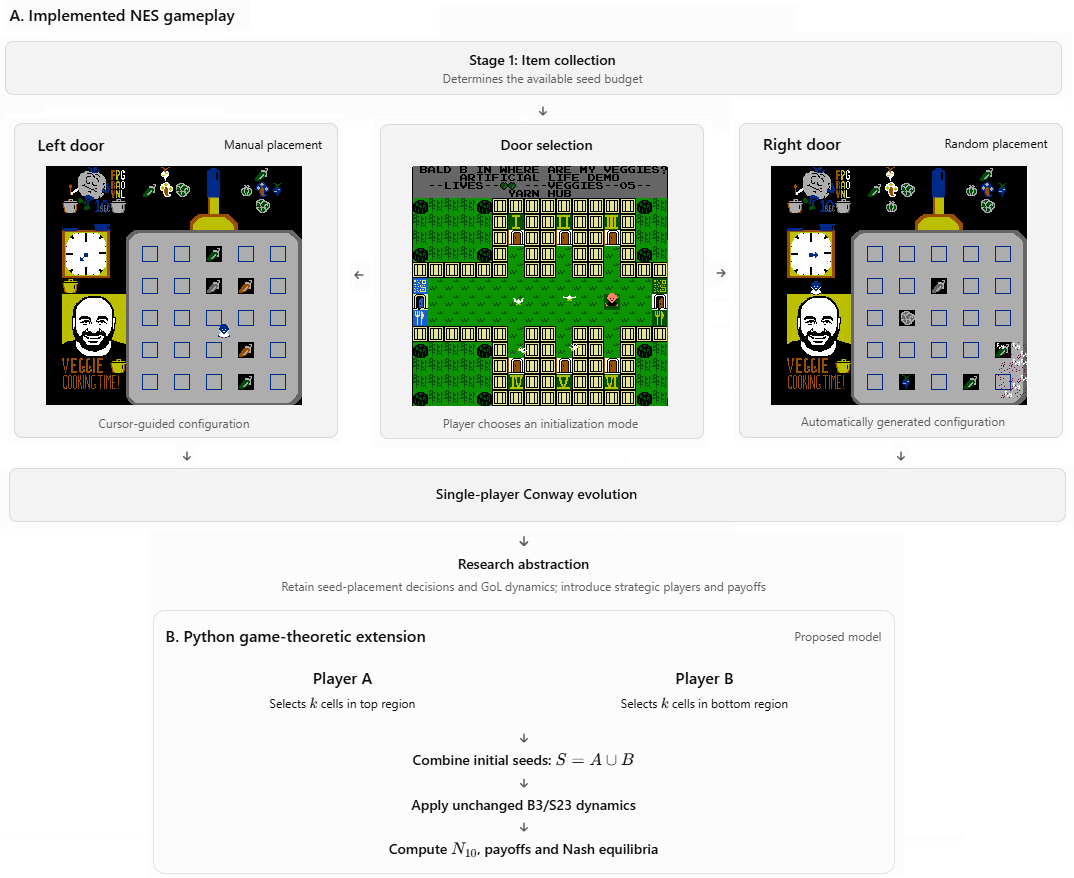
\includegraphics[width=1.0\linewidth]{figures/fig10_nes_initialization_modes.png}
\caption{NES mode-selection interface: manual placement (blue door) and random initialization (brown door). The screen belongs to the single-player interface, not to the two-player game-theoretic extension.}\label{fig:nesmodes}
\end{figure}

\begin{figure}[H]
\centering
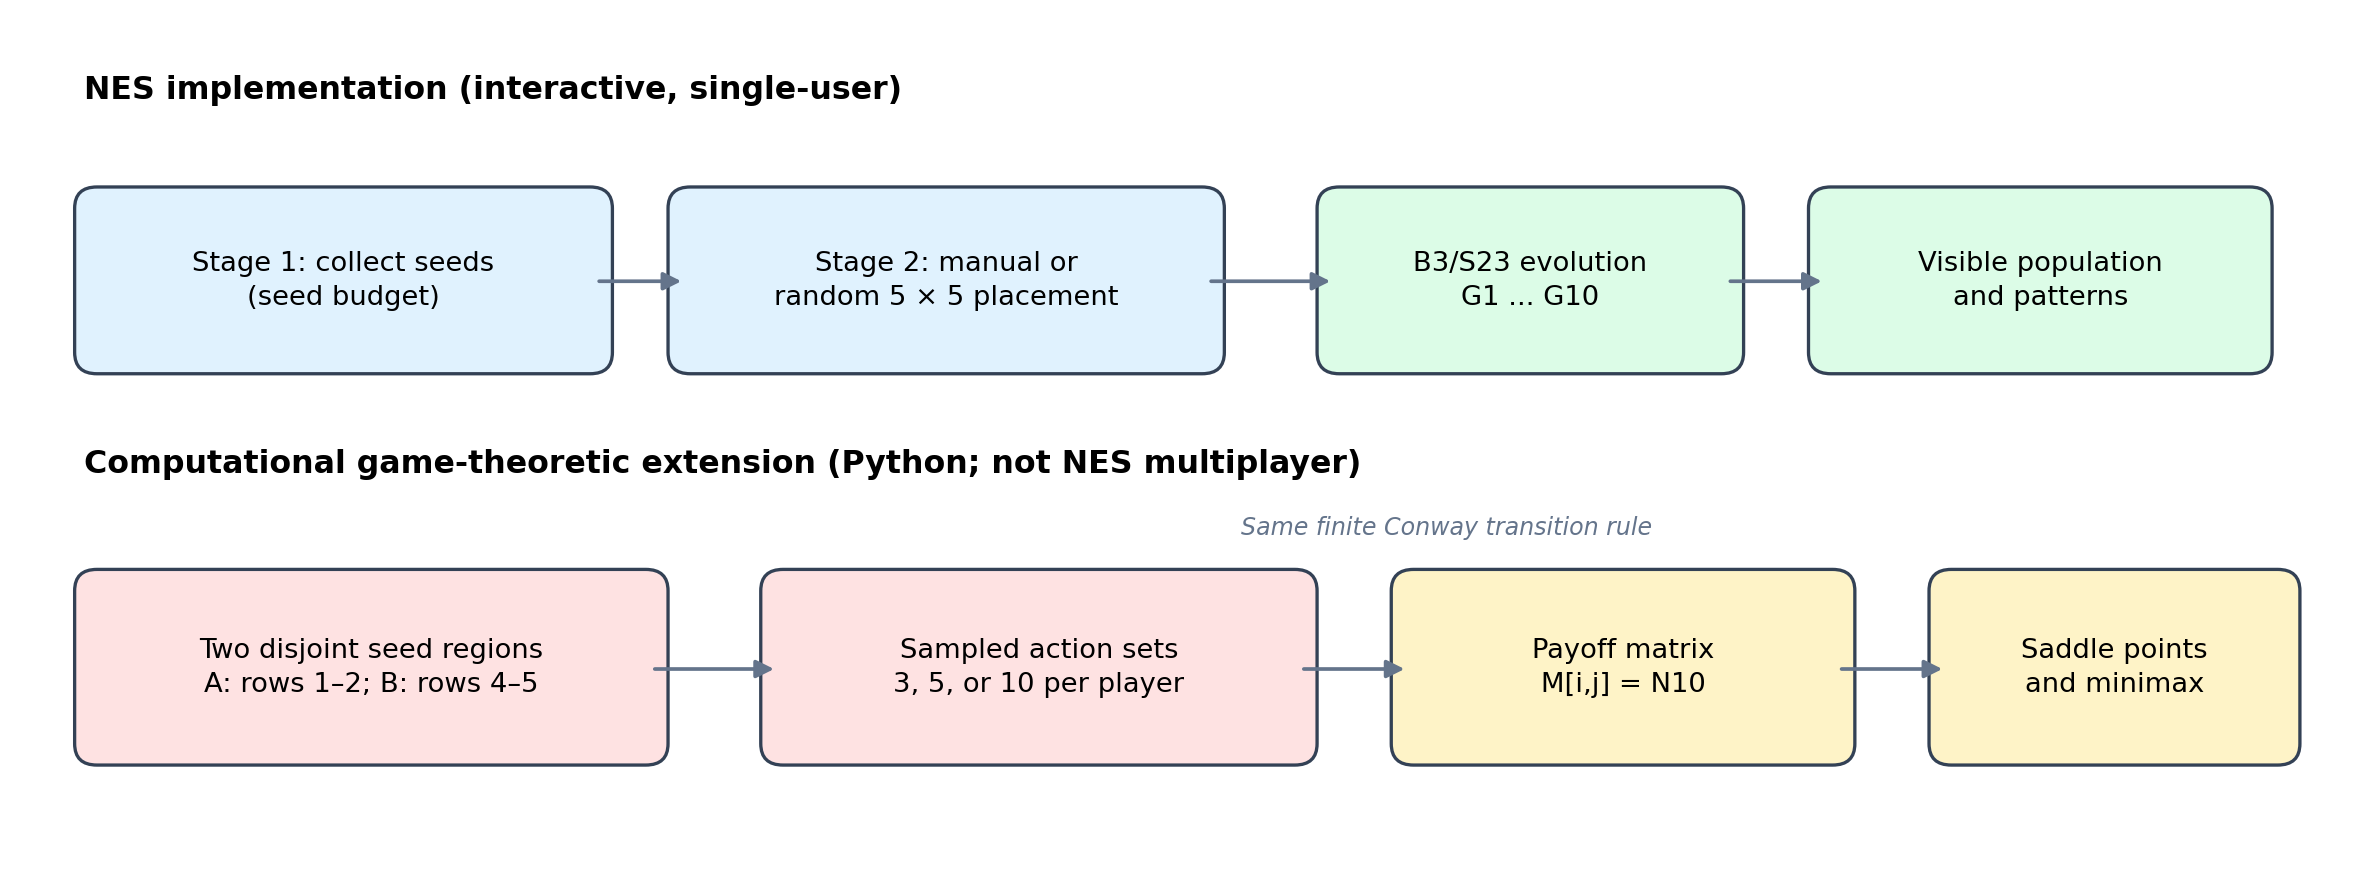
\includegraphics[width=\linewidth]{figures/fig01_nes_to_formal_model.png}
\caption{Relationship between the implemented NES gameplay and the proposed game-theoretic extension. \emph{Top:} the original single-player NES workflow. After collecting items that determine the available seed budget, the player chooses between two doors: the left door leads to manual seed placement, while the right door activates random initialization. Both modes produce an initial $5\times5$ configuration that evolves according to Conway's B3/S23 rules. \emph{Bottom:} the separate Python-based two-player zero-sum model, in which two players independently select fixed-cardinality seed patterns within disjoint regions. Their combined initial configuration undergoes the same Conway dynamics, and the terminal live-cell population determines the payoff matrix used for Nash-equilibrium analysis. The lower panel represents a mathematical extension and is not a multiplayer feature of the NES implementation.}
\label{fig:framework}
\end{figure}

\subsection{Finite Cellular Automaton and Outcome Variable}

Let $\mathcal{C}=\{1,\ldots,5\}\times\{1,\ldots,5\}$ be the board and let $x_t(c)\in\{0,1\}$ indicate the live/dead state of cell $c$ at recorded generation $t$. Cells outside $\mathcal{C}$ are always considered dead (finite, nonwrapping boundaries). For each cell $c$, let $n_t(c)$ denote the number of live Moore-neighborhood cells at generation $t$, excluding $c$ itself. The conventional synchronous B3/S23 update is
\begin{equation}\label{eq:conway}
x_{t+1}(c)=
\begin{cases}
1, & n_t(c)=3,\\
x_t(c), & n_t(c)=2,\\
0, & \text{otherwise.}
\end{cases}
\end{equation}
We call the configured initial board \emph{Generation 1}. The final observation, \emph{Generation 10}, is reached after exactly nine synchronous applications of Equation~\eqref{eq:conway}. This explicit convention avoids an off-by-one difference when comparing trajectories across programming platforms. Write $F^{9}(S)$ for the configuration reached after nine updates from initial live-cell set $S\subseteq\mathcal{C}$, and define the terminal population
\begin{equation}\label{eq:outcome}
f(S)=N_{10}(S)=\bigl|F^{9}(S)\bigr|,\qquad 0\leq f(S)\leq25.
\end{equation}
The terminal population $N_{10}$ is \emph{not} equivalent to trajectory persistence, whether persistence is measured by surviving generations or by final nonextinction. The primary zero-sum game is defined solely through $N_{10}$.

\subsection{Exploratory Persistence and Behavioral Classification}

For the single-player initialization analyses, let $S_t$ denote the set of live cells at recorded generation $t$, and let $N_t=|S_t|$ denote the corresponding number of live cells. We use the indicator function $\mathbf{1}\{P\}$, defined for any logical statement $P$ as
\begin{equation}\label{eq:indicator}
\mathbf{1}\{P\}=
\begin{cases}
1, & \text{if }P\text{ is true},\\
0, & \text{if }P\text{ is false}.
\end{cases}
\end{equation}
Using this notation, we distinguish the terminal survival indicator $I_{10}=\mathbf{1}\{N_{10}>0\}$ from the finite-window count
\begin{equation}\label{eq:survival_window}
L=\sum_{t=1}^{10}\mathbf{1}\{N_t>0\}.
\end{equation}
The terminal survival indicator $I_{10}$ equals one if at least one cell remains alive in the final recorded generation, and zero otherwise. In contrast, $L$ counts the number of recorded generations containing at least one live cell. The quantity $N_{10}$ measures the number of live cells in the final recorded state.
Under standard Conway dynamics, the empty state is absorbing: once all cells are dead, no new live cells can emerge. Consequently, $L$ also represents the number of nonempty recorded generations before extinction, up to the ten-generation observation limit. For an initially nonempty board, $L\in\{1,\ldots,10\}$.

The exploratory analysis also distinguishes fixed states ($S_{t+1}=S_t$), oscillatory trajectories (a previously visited state recurs with period greater than one), and trajectories with no observed recurrence during the finite window. A trajectory without observed recurrence is termed \emph{nonrepeating within the observation window}, rather than proven aperiodic. These labels are descriptive and do not enter the zero-sum utility function. Related cellular-automaton treatments include \citet{ilachinski2001cellular} and \citet{adamatzky2010game}.

\subsection{Disjoint Placement Regions and Feasible Seed Patterns}

To represent independent initial placement decisions while keeping each player's contribution identifiable, we assign the players separate regions of the board. The empty central row acts as a one-row buffer between their initial placements, preventing overlap and separating the two seed patterns at the start of the game. This is a modeling assumption about initialization; it does not imply permanent ownership of any cells. 

Define $\mathcal{R}_A=\{1,2\}\times\{1,\ldots,5\}$ and $\mathcal{R}_B=\{4,5\}\times\{1,\ldots,5\}$. Player A may seed $\mathcal{R}_A$ only, and Player B may seed  $\mathcal{R}_B$ only; row 3 is initially empty. After the initial configuration is formed, the automaton evolves on the complete $5\times5$ board, and newly born cells may occupy any row.

For $k\in\{3,4,5,6,7\}$, each player's full \emph{region-constrained} action space is
\begin{equation}
\mathcal{A}_k=\{A\subseteq\mathcal{R}_A:|A|=k\},\qquad
\mathcal{B}_k=\{B\subseteq\mathcal{R}_B:|B|=k\}.
\end{equation}
Both regions contain ten feasible sites, hence $|\mathcal{A}_k|=|\mathcal{B}_k|=\binom{10}{k}$, reaching 252 at $k=5$. We do \emph{not} solve all $\binom{10}{k}^2$ action profiles for each budget. Instead, the reported equilibrium analysis concerns explicitly sampled subgames with $m$ available actions per player, where $m\in\{3,5,10\}$.

\subsection{Primary Zero-Sum Model, Saddle Points, and Mixed Equilibria}

For an ordered sampled collection $(A_1,\ldots,A_m)$ for the maximizing player and $(B_1,\ldots,B_m)$ for the minimizing player, the payoff matrix is
\begin{equation}\label{eq:matrix}
M_{ij}=f(A_i\cup B_j),\qquad u_A(i,j)=M_{ij},\quad u_B(i,j)=-M_{ij}.
\end{equation}
The antagonistic utilities represent a controlled mathematical question: how strategic placement affects final live-cell population under competing preferences. They should \emph{not} be interpreted as survival of A-owned versus B-owned organisms, because no ownership is propagated by the B3/S23 rule.

A pure Nash equilibrium occurs when a matrix entry is simultaneously the maximum in its column and the minimum in its row:
\begin{equation}\label{eq:saddle}
M_{i^*j^*}=\max_i M_{ij^*}=\min_j M_{i^*j}.
\end{equation}
Equivalently, the pure-strategy maximin and minimax coincide. With $p,q\in\Delta_m$ the players' mixed strategies, the mixed game value is
\begin{equation}\label{eq:minimax}
v(M)=\max_{p\in\Delta_m}\min_{q\in\Delta_m}p^{\mathsf T}Mq
=\min_{q\in\Delta_m}\max_{p\in\Delta_m}p^{\mathsf T}Mq.
\end{equation}
We solve the primal and dual linear programs using the HiGHS method accessed through SciPy\texttt{.linprog} \citep{vonNeumann1944,nash1951,virtanen2020}. A finite zero-sum game always has a mixed equilibrium; thus ``no pure equilibrium'' never means ``no Nash equilibrium.'' For each computed matrix, we store the value, a representative optimal mixed-strategy pair, support sizes, pure saddle-point count, and primal--dual gap.

\subsection{Secondary Counterfactual-Contribution Model}

To distinguish antagonistic competition from a distinct interpretation of individual contributions, an exploratory secondary model considers
\begin{equation}\label{eq:marginal}
\widetilde u_A(A,B)=f(A\cup B)-f(B),\qquad
\widetilde u_B(A,B)=f(A\cup B)-f(A).
\end{equation}
This is \emph{not} a second formulation of the zero-sum game and not a biological-ownership game. In fact, it has a useful formal property.

\begin{Proposition}\label{prop:potential}
For fixed feasible action sets, the game defined by Equation~\eqref{eq:marginal} is an exact potential game with potential $\Phi(A,B)=f(A\cup B)$.
\end{Proposition}
\begin{proof}
For a unilateral change from $A$ to $A'$ with $B$ fixed, the $-f(B)$ term cancels, so $\widetilde u_A(A',B)-\widetilde u_A(A,B)=\Phi(A',B)-\Phi(A,B)$. The analogous difference for player B cancels $-f(A)$. Hence every unilateral utility change is precisely the corresponding potential change, which establishes the claim by the exact-potential definition \citep{monderer1996}.
\end{proof}

The proposition implies that at least one pure equilibrium exists in every finite restriction of the \emph{secondary} model (a maximizer of $\Phi$). Results for this model are reported only as supplementary context in the initial deterministic and robustness experiments. All headline no-pure-equilibrium rates refer to the primary zero-sum model.

\subsection{Experimental Program and Relationship among Analyses}\label{sec:roadmap}

The complete research program proceeds from the interactive platform and descriptive initial-condition experiments to strategic matrix games and their controls. To make the relationship among the eight numbered computational phases explicit, we distinguish: Phase 1, the NES-based interactive implementation and seed-placement workflow \citep{senzio2026nes}; Phase 2, exploratory manual-versus-random placement, finite-horizon persistence, and spatial-pattern characterization; Phase 3, the expanded density survey; Phase 4, deterministic three-action payoff matrices; Phase 5, independently sampled random three-action robustness games; Phase 6, paired spatial-transformation sensitivity; Phase 7, nested strategy-action scaling; and Phase 8, within-matrix payoff-permutation controls. The NES--Python state-transition comparison is a separate cross-platform validation component rather than a ninth equilibrium experiment.

The first two components characterize how initial conditions influence the automaton without two-player strategic payoffs. Phases 4--8 examine restricted strategic games built from those dynamics; Phase 3 supplies additional density context. Cross-platform comparison checks selected state trajectories independently of the equilibrium optimizer. Thus the persistence statistic $L$, terminal nonextinction $I_{10}$, and strategic payoff $N_{10}$ remain distinct throughout.

\subsection{Computational Experiments and Sampling}\label{sec:phases}

The numerical study was organized into complementary designs; the designs are not interchangeable replications and their outcome counts must not be pooled as if they were independent. The separation of experimental units, controlled factors, and descriptive versus comparative outcomes follows general simulation-study and experimental-design principles \citep{law2015simulation,montgomery2017design}. These references provide methodological context, not a post hoc justification for the chosen replication counts.

\begin{table}[H]
\centering
\caption{Computational designs used to characterize or validate the strategic model. ``Pairings'' denotes deterministic joint action profiles, not independent random samples.}\label{tab:designs}
\begin{tabularx}{\linewidth}{@{}lXrr@{}}
\toprule
\textbf{Design} & \textbf{Experimental unit and purpose} & \textbf{Games} & \textbf{Pairings}\\
\midrule
Density survey & 100 initial configurations for each density 1--25; background, not the central equilibrium analysis & --- & 2,500 runs\\
Deterministic templates & One 3$\times$3 strategic matrix at each budget 3--6 & 4 & 36\\
Random 3$\times$3 robustness & 100 independently sampled three-action strategy sets per budget 3--7 & 500 & 4,500\\
Spatial transformations & 40 independent strategy sets per budget, each evaluated under 16 paired transformation combinations & 3,200 & 28,800\\
Nested action-set scaling & 100 independent ten-action sets per budget, yielding paired 3$\times$3, 5$\times$5, 10$\times$10 subgames & 1,500 & 67,000\\
Permuted-payoff control & 200 independent permutations of each of the 1,500 scaling matrices & 300,000 controls & ---\\
NES comparison & 10 selected initial configurations, 10 observed generations each & --- & 100 states\\
\bottomrule
\end{tabularx}
\end{table}

In the exploratory density survey, 100 configurations with exactly $n$ initial live cells were sampled uniformly for each $n\in\{1,\ldots,25\}$. For the strategic experiments, budgets were restricted to $k=3,\ldots,7$, yielding initial density $2k/25$. The density survey supplies contextual motivation rather than evidence of an optimal strategic budget.

\paragraph{Exploratory initialization protocol.}
A complementary exploratory experiment characterized finite-horizon persistence under random and manually specified initialization. This protocol is distinct from the 100-per-density survey reported above. In this exploratory protocol, 10 random initial configurations were generated per density ($n=1,\ldots,25$), and at the selected density $n=12$, 40 manually constructed configurations were evaluated (10 in each of four descriptive spatial families: clustered, linear, dispersed, and semi-structured). A separate set of 10 random configurations at $n=12$ was used for the direct manual--random comparison. For this dataset, the reported persistence measure is the number of recorded generations with nonempty states within the ten-generation observation window; final-generation survival is recorded separately as $\mathbf{1}\{N_{10}>0\}$. These descriptive experiments did not sample competing player strategies and were not included in the 1,500 zero-sum games. Their purpose here is to establish the motivation for investigating placement geometry at a fixed seed count. The exploratory summary statistics require verification against original run-level records before submission; they are not pooled with the larger density survey or with the strategic games.


In the deterministic-template analysis, we chose three operationally defined spatial families per player---compact, row-oriented, and dispersed---for budgets three through six. The resulting four $3\times3$ games illustrate how equilibria and mixed values arise, but a single family per budget cannot establish population-level trends.

For sampled robustness games, each action is a uniformly selected fixed-cardinality subset of its corresponding ten-cell placement region; the three distinct actions per player are drawn without replacement. One hundred independent sets were created for each budget, using master pseudorandom seed 20261020. This design investigates variation across \emph{sampled restricted subgames}, not across an exhaustive strategic space.

In the spatial experiment, forty independent three-action sets per budget were subjected to sixteen paired combinations of four within-region transformations: identity, horizontal reflection, one-column cyclic shift, and row swap. These operations change feasible seed coordinates but are not necessarily global symmetries of the full Conway domain. Transformations from the same original set are paired and statistically dependent.

The main scaling experiment sampled ten distinct region-constrained actions per player for each of 100 independent sets and each budget. The upper-left $3\times3$ and $5\times5$ submatrices of a common $10\times10$ payoff matrix were analyzed alongside the full sampled matrix. Consequently, action-size comparisons within the same sampled set are \emph{nested paired comparisons}. One hundred such sets per budget yield $5\times100\times3=1{,}500$ matrix games, containing $(3^2+5^2+10^2)\times500=67{,}000$ payoff entries, some of which are reused across nested subgames. The board size never changes in this scaling experiment.

\subsection{Tie-Preserving Permutation Controls}\label{sec:permutation_method}

Terminal live-cell counts are integer-valued, so different matrix entries can have equal payoffs. Analytical saddle-point probabilities derived under continuous independent entries, for example \citet{thorp1979}, are therefore not a direct null for the observed matrices. For every empirical matrix $M$, we generate $200$ controls by uniformly permuting its $m^2$ entries and reshaping the result to $m\times m$. Let $\pi$ be a random permutation of the flattened matrix indices, and let $M^{\pi}$ denote the reshaped control. Then
\begin{equation}
\{M^{\pi}_{ij}:1\le i,j\le m\}_{\mathrm{multiset}}
=
\{M_{ij}:1\le i,j\le m\}_{\mathrm{multiset}}.
\end{equation}
Thus, each control preserves the empirical payoff multiset, its mean and variance, and the occurrence of payoff ties, while disrupting the row--column organization. For each empirical matrix, we compare the observed binary indicator for absence of a pure equilibrium with the Monte Carlo rate of this outcome across its $200$ controls. For each budget and action count, the mean difference is computed across \emph{100 original games}; the $20{,}000$ permutations are not treated as independent observations.

Uncertainty intervals for paired differences use 4,000 game-level bootstrap resamples. Exploratory two-sided $p$-values are generated by approximating a conditional permutation null with independent Bernoulli draws parameterized by each game's estimated control rate; these values are approximate, unadjusted for the 15 displayed comparisons, and omitted from the main confirmatory interpretation. A smaller subset of permuted matrices is used for descriptive control minimax values. A difference between the observed outcomes and the within-matrix permutation controls indicates that row--column organization is associated with the outcome relative to random arrangements of the same payoff values. This comparison does \emph{not} isolate cellular dynamics as the only causal mechanism, because sampling, top/bottom placement, and shared action sets also induce structure.

\subsection{NES--Python State-Transition Comparison}\label{sec:validation_method}

Ten initial states were selected from strategic configurations investigated in the spatial and scaling experiments. Their initial positions were placed in the NES GoL interface, where all initially live cells became indistinguishable once the board was configured. For each case, the ten displayed/recorded generations were transcribed as five binary row strings and compared cell-by-cell with the independently generated Python trajectory. The comparison tested \emph{the complete $5\times5$ state}, rather than only the number of survivors.

The comparison covers ten configurations and ten recorded states per configuration: $10\times10=100$ full boards, containing $100\times25=2{,}500$ binary observations. This is a selected-case validation of the state-transition implementation and corresponding terminal populations, not validation of Nash-optimal mixed strategies or of every sampled action profile.

\section{Results}\label{sec:results}

\subsection{Density-Dependent Persistence and Finite-Horizon Dynamics}\label{sec:density}

We characterized initial-density effects in two separate computational sampling protocols, both using a $5\times5$ board and ten recorded generations. The exploratory protocol drew ten uniformly sampled initial configurations at each density $n=1,\ldots,25$ (250 runs total). Its density-resolved persistence curve is reproduced in Figure~\ref{fig:densityexploratory}; the ordinate represents the recorded finite-horizon persistence statistic, not the number of live cells at Generation 10. The figure is retained as an exploratory visualization, and its plotted values should be reconciled with the original run-level data before submission. The fixed sample size of ten per density does not support a precise estimate of an optimal density.

\begin{figure}[H]
\centering
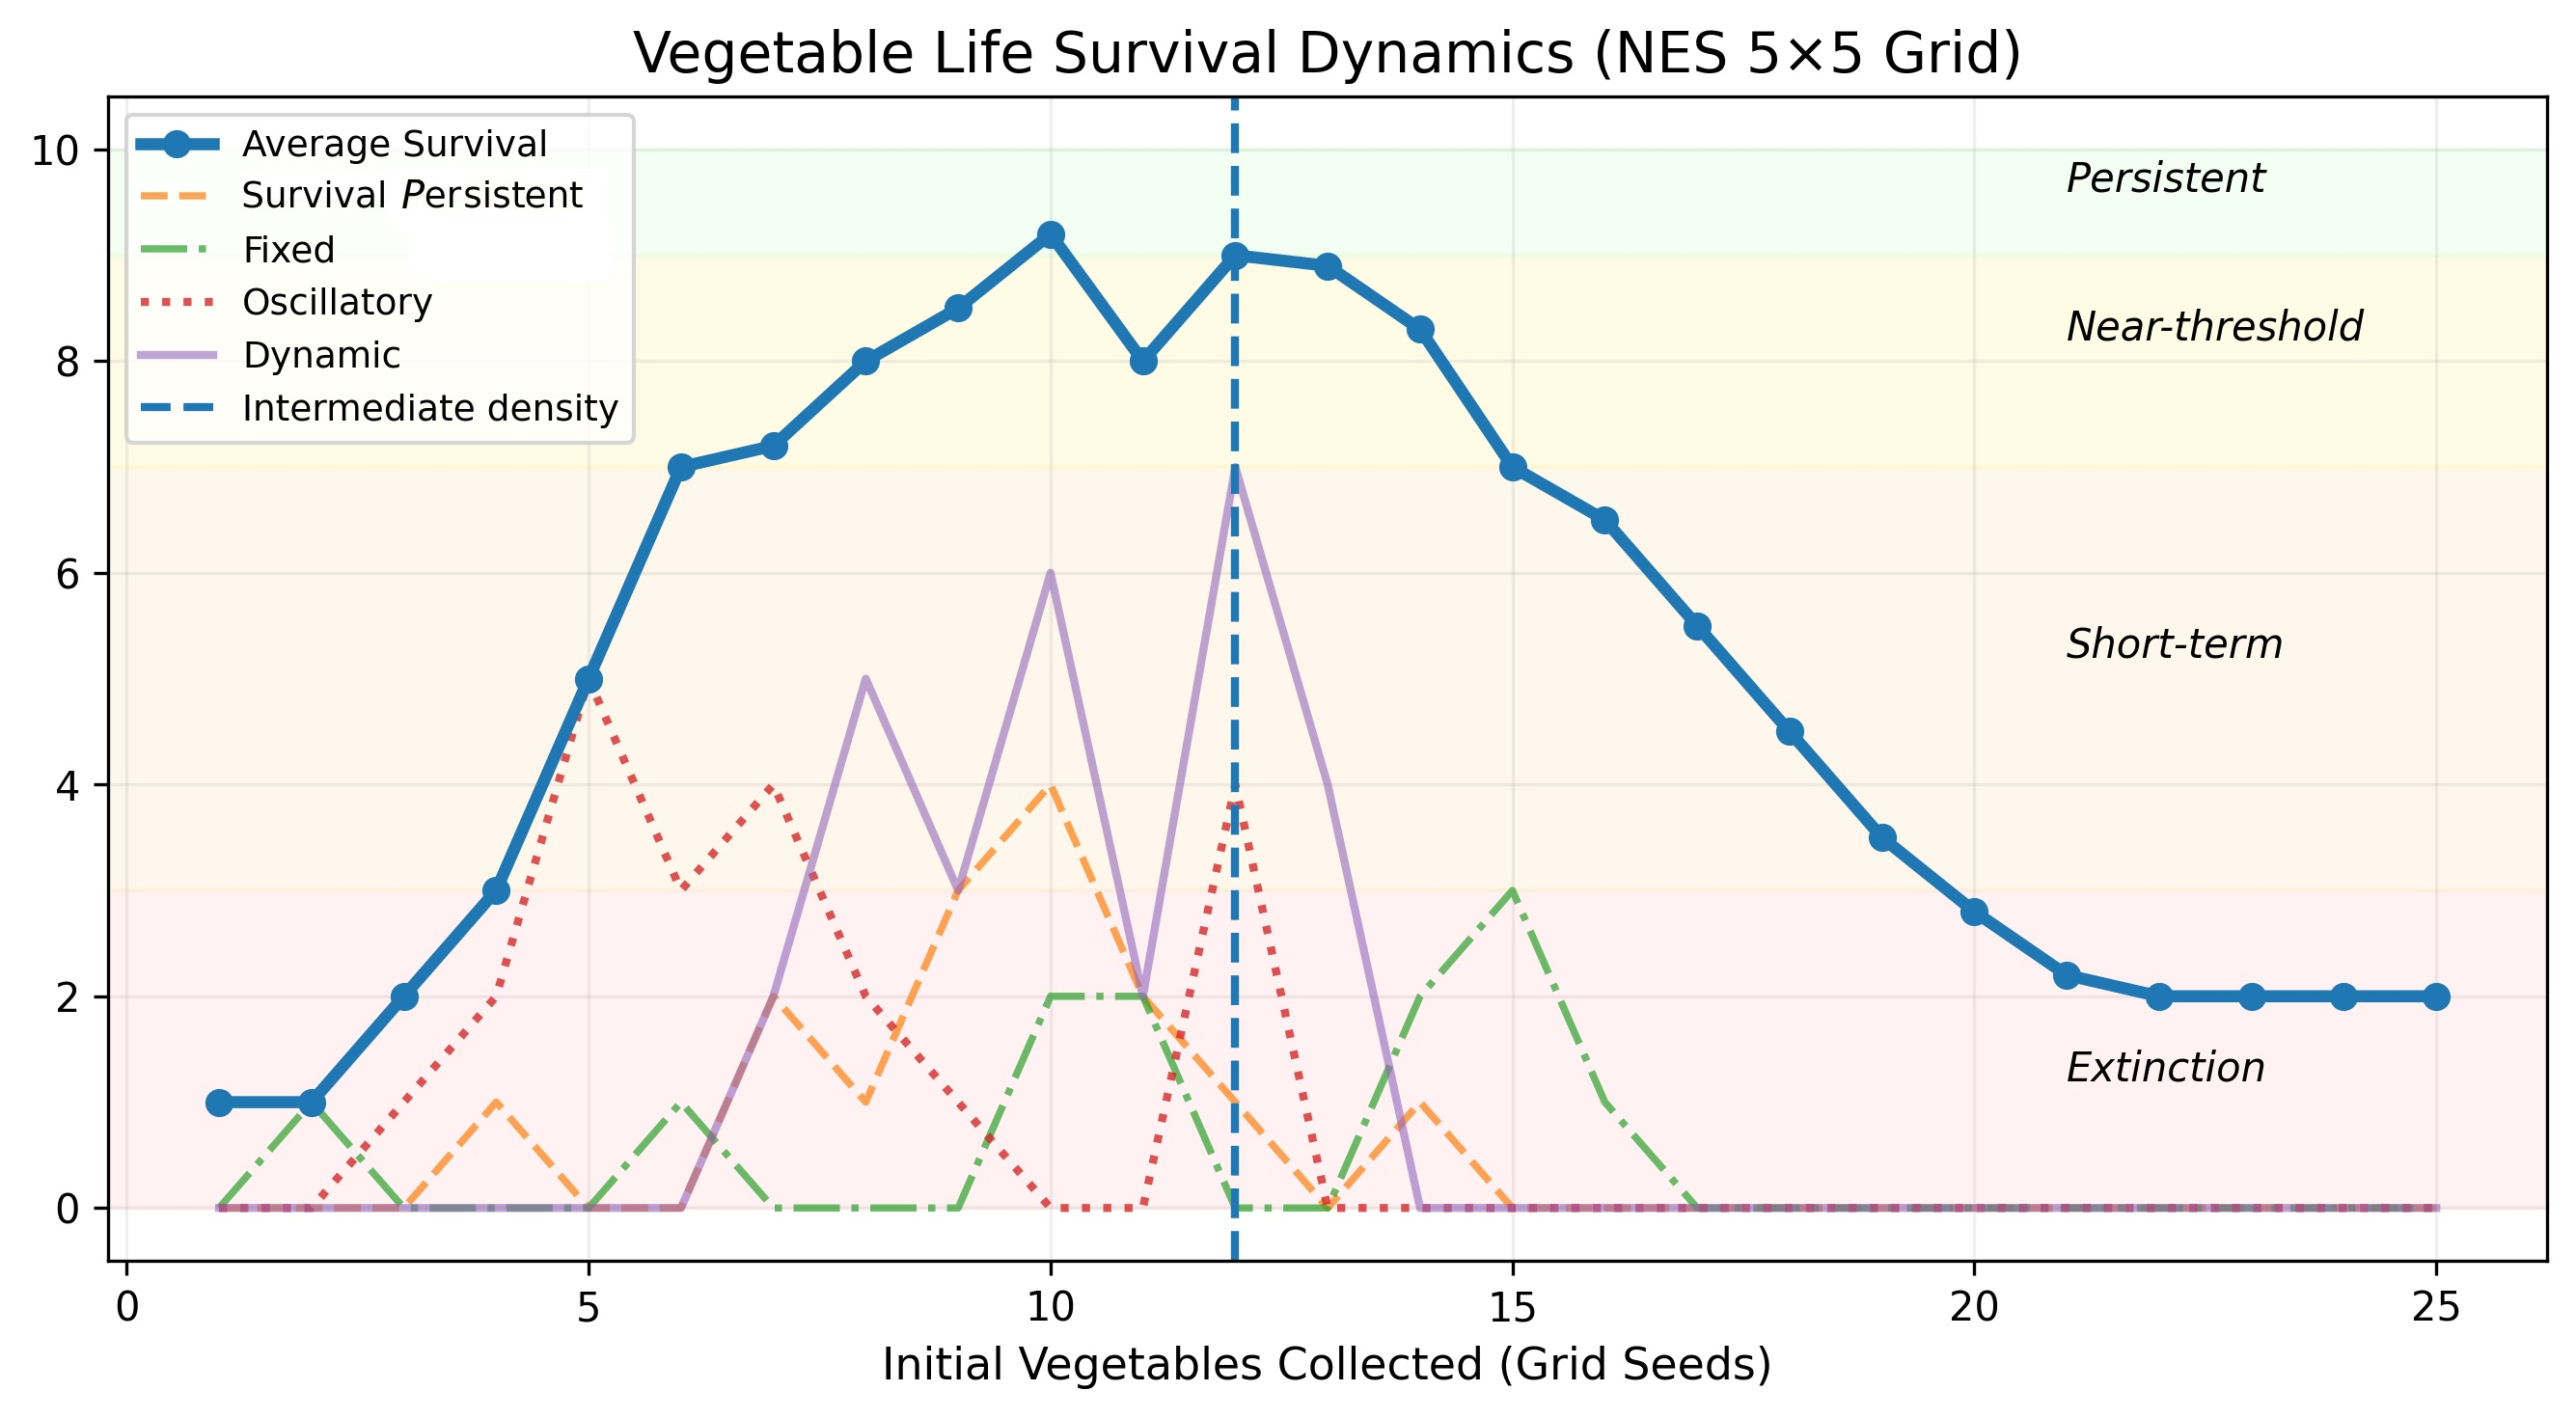
\includegraphics[width=.84\linewidth]{figures/fig11_density_persistence_exploratory.png}
\caption{Exploratory density-dependent persistence under random initialization on the finite $5\times5$ board (ten configurations per initial density).}\label{fig:densityexploratory}
\end{figure}

A larger, independently sampled survey comprised 100 configurations at each of the 25 densities, for 2,500 finite-horizon runs and 25,000 recorded board states. In this larger survey, the largest observed mean count of nonempty recorded generations was 8.57 at initial density 13, while the highest empirical frequency of a nonempty Generation 10 was 63\% at densities 10 and 11. These distinct measures should not be conflated: the former summarizes duration within the observation window, the latter is the binary terminal survival indicator, and neither equals the primary game-theoretic payoff $N_{10}$.

The density-dependent patterns motivate controlling seed budgets and examining spatial arrangement. Together with the manual-versus-random placement experiment, these results provide the descriptive initial-condition component of the unified study, whereas the subsequent analyses introduce explicit competing agents and game-theoretic payoffs. They do not imply that any density is a Nash equilibrium, nor that the density with the greatest mean persistence maximizes the terminal population under competitive placement.

\subsection{Exploratory Single-Player Spatial Initialization Results}
\label{sec:exploratory_spatial}
The exploratory manual-placement experiment compared 40 manually specified initial configurations at a fixed total density of 12 live cells. Four spatial families were represented by ten distinct configurations each (Figure~\ref{fig:manualfamilies}). The descriptive outcomes are reproduced in Table~\ref{tab:manualfamilies}. At this common density, linear and semi-structured configurations had higher average numbers of nonempty recorded generations than clustered and dispersed configurations. These labels describe manually constructed configurations; they are not the action families or equilibrium strategies of the two-player model.

\begin{figure}[H]
\centering
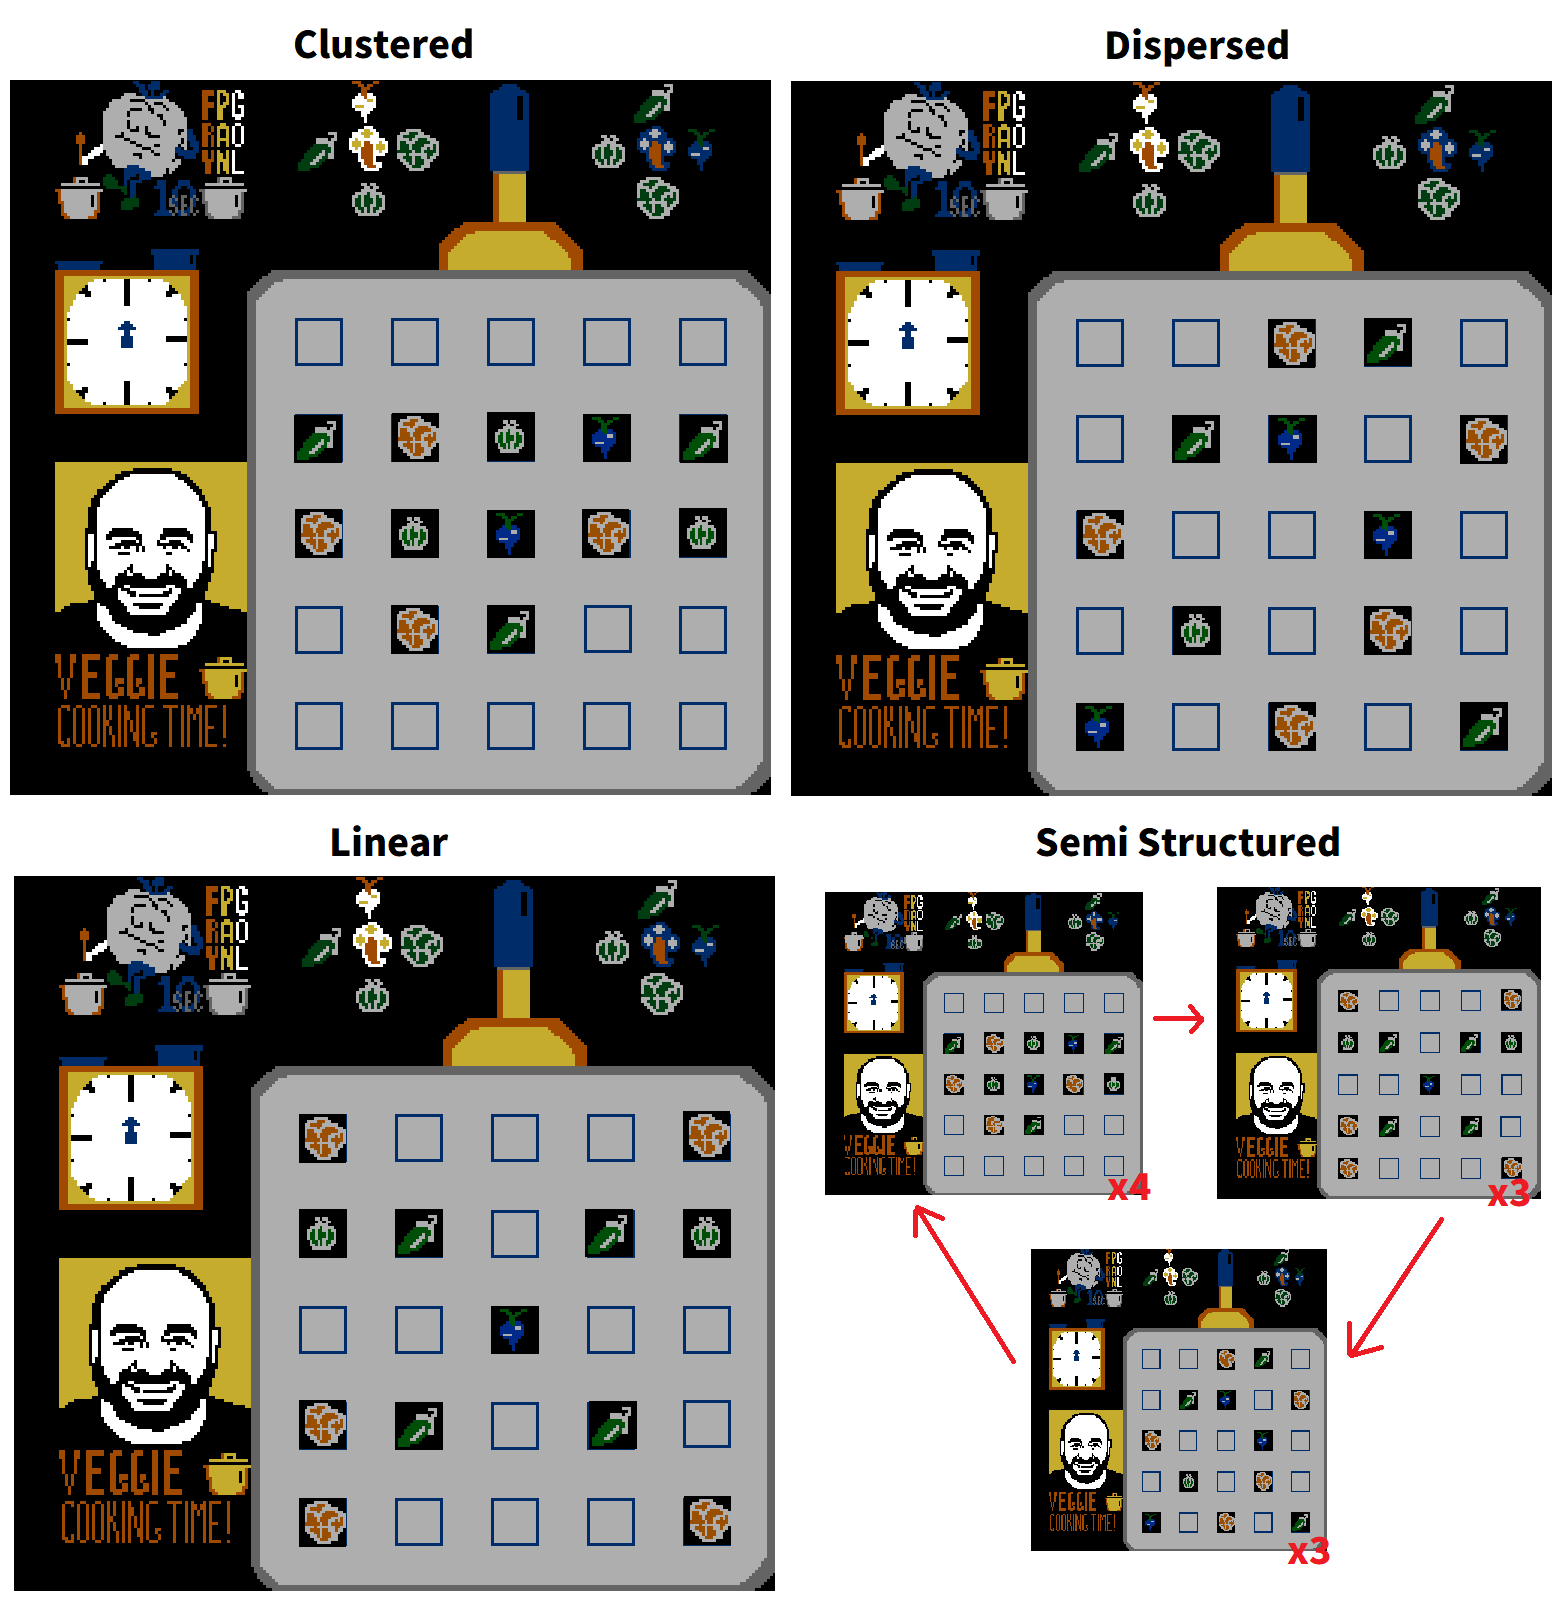
\includegraphics[width=.68\linewidth]{figures/fig08_manual_spatial_patterns.png}
\caption{Illustrative manual-placement patterns on the finite $5\times5$ Game of Life board. Each panel shows an initial configuration with 12 live cells: a compact cluster, a line, a dispersed arrangement, or a semi-structured arrangement with some local grouping but no single dominant cluster or straight-line form. These examples provide methodological context and are not computed Nash strategies.}\label{fig:manualfamilies}
\end{figure}

\begin{table}[H]
\centering
\caption{Exploratory manual-placement results from the single-player initialization study at initial density 12; ten configurations per category. ``Reaching Generation 10'' is a terminal nonextinction indicator, distinct from the average count of nonempty recorded generations. These descriptive summaries have not been independently re-estimated from run-level records in the present draft.}\label{tab:manualfamilies}
\begin{tabular}{lcc}
\toprule
\textbf{Spatial family} & \textbf{Mean nonempty generations} & \textbf{Reaching G10 (\%)}\\
\midrule
Clustered & 6.8 & 20\\
Linear & 8.8 & 70\\
Dispersed & 6.2 & 10\\
Semi-structured & 9.0 & 60\\
\bottomrule
\end{tabular}
\end{table}

In the same exploratory experiment, ten random configurations at density 12 yielded a mean of $9.1\pm1.45$ recorded generations, whereas the 40 manually designed configurations yielded $7.7\pm1.65$ (reported mean $\pm$ standard deviation; Figure~\ref{fig:manualrandom}). This is a descriptive comparison of unequal, nonrandomly selected groups, not evidence that random initialization is universally superior to manual placement. In particular, no hypothesis test, random assignment of manual patterns, or human-subject experiment was reported. Its relevance to the present game-theoretic analysis is narrower but useful: equal seed counts can produce different outcomes under different spatial arrangements.

\begin{figure}[H]
\centering
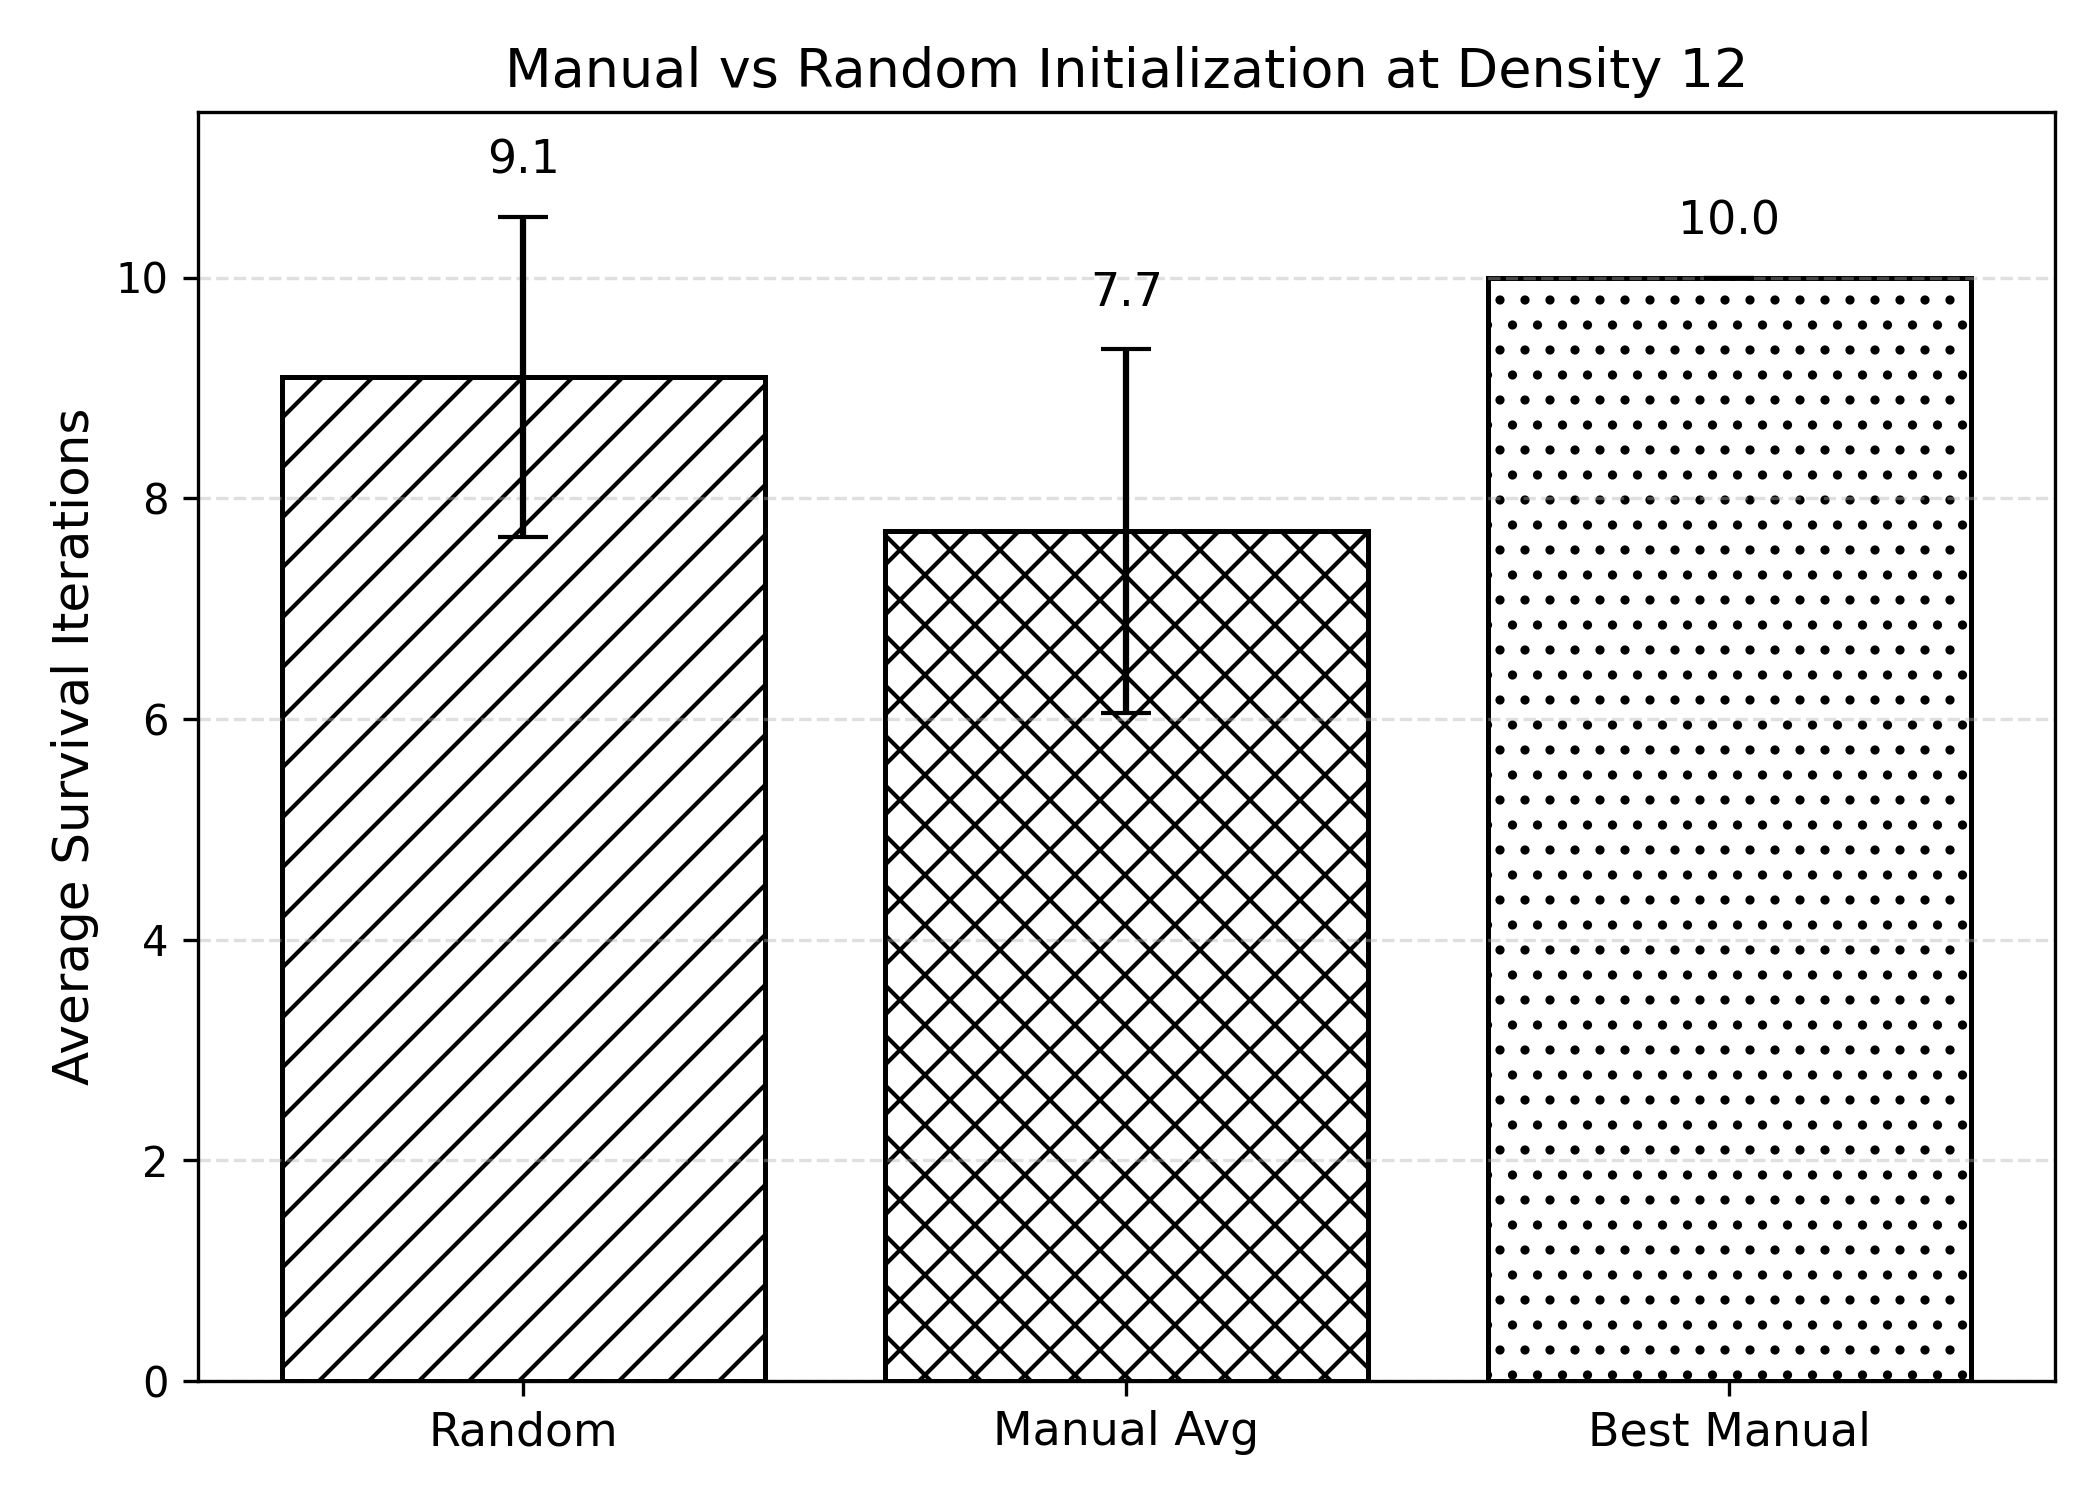
\includegraphics[width=.72\linewidth]{figures/fig09_manual_vs_random_exploratory.png}
\caption{Exploratory comparison at initial density 12, with random initialization ($n=10$) and manually constructed patterns ($n=40$). Error bars represent reported standard deviations. This figure summarizes single-player persistence, not terminal population payoffs or strategic equilibrium performance.}\label{fig:manualrandom}
\end{figure}

\subsection{Deterministic Payoff Matrices}

The deterministic-template experiment yielded zero-sum pure saddle points at budgets 3, 4, and 6 (three saddle entries in each matrix), but no pure saddle point at budget 5. The value of the latter $3\times3$ game was approximately $3.158$ final live cells, and its equilibrium was mixed. Figure~\ref{fig:example} illustrates this particular restricted-game example. It does not identify a universal transition at budget five: changing the chosen strategy patterns can change the existence of a pure equilibrium.

\begin{figure}[H]
\centering
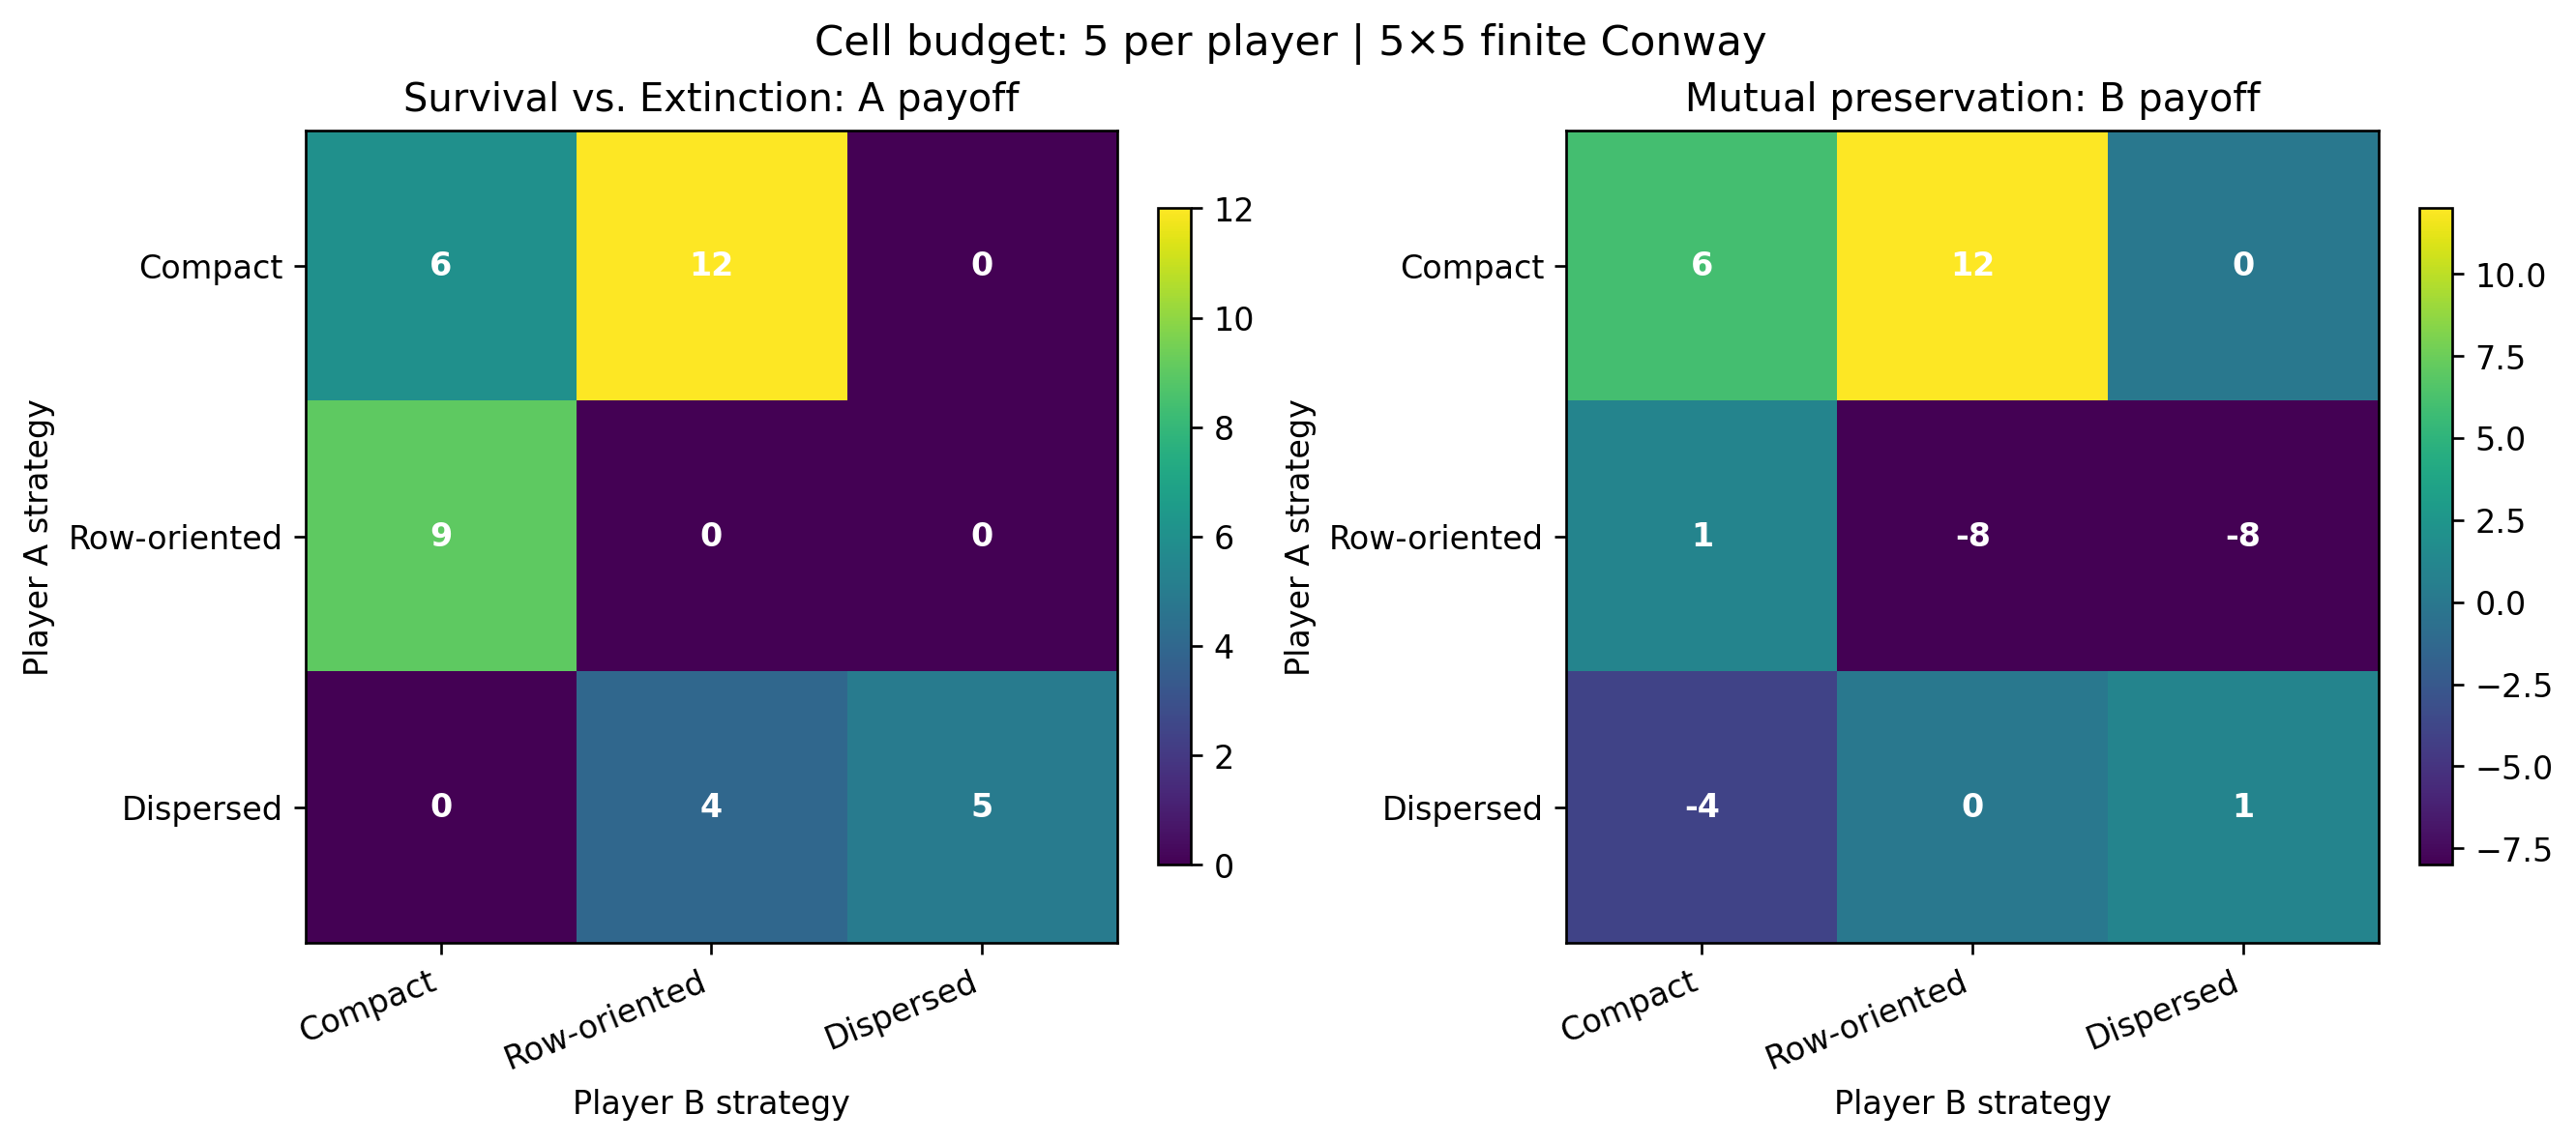
\includegraphics[width=.95\linewidth]{figures/fig02_deterministic_budget5_payoff.png}
\caption{Budget-five deterministic three-action example. Left: primary zero-sum payoff $M_{ij}=N_{10}$ for maximizing player A; opposing player B receives $-M_{ij}$. Right: player B's separate counterfactual-contribution payoff from the secondary potential game (Equation~\eqref{eq:marginal}). The primary matrix has no pure saddle point; its mixed-game value is approximately 3.158 live cells.}\label{fig:example}
\end{figure}

\subsection{Independent Random Three-Action Games}

Among one hundred independently sampled $3\times3$ restricted zero-sum games at each budget, the proportion lacking a pure equilibrium was 12\%, 32\%, 42\%, 38\%, and 57\% for budgets three through seven, respectively. The corresponding mean mixed minimax values were 0.944, 2.514, 2.280, 2.408, and 3.541 terminal live cells. These budget-indexed estimates are nonmonotonic, and the finite sample provides no basis to assign a universal ``critical'' seed budget. The results show that pure-equilibrium existence varies substantially across the randomly sampled strategy configurations even when the board size and dynamics are fixed.

\subsection{Sensitivity to Spatial Transformations}

Across the spatial-transformation design, 3,200 transformed $3\times3$ matrix games were evaluated: 40 original sets per budget, each under 16 transformation combinations. The observed no-pure-equilibrium rates were 12.3\%, 47.3\%, 39.2\%, 45.0\%, and 55.9\% for budgets 3--7. The fraction of original sets for which equilibrium status changed between at least two transformations was 65.0\%, 100\%, 97.5\%, 100\%, and 100\%, respectively. Figure~\ref{fig:spatial} displays the budget-specific rates.

\begin{figure}[H]
\centering
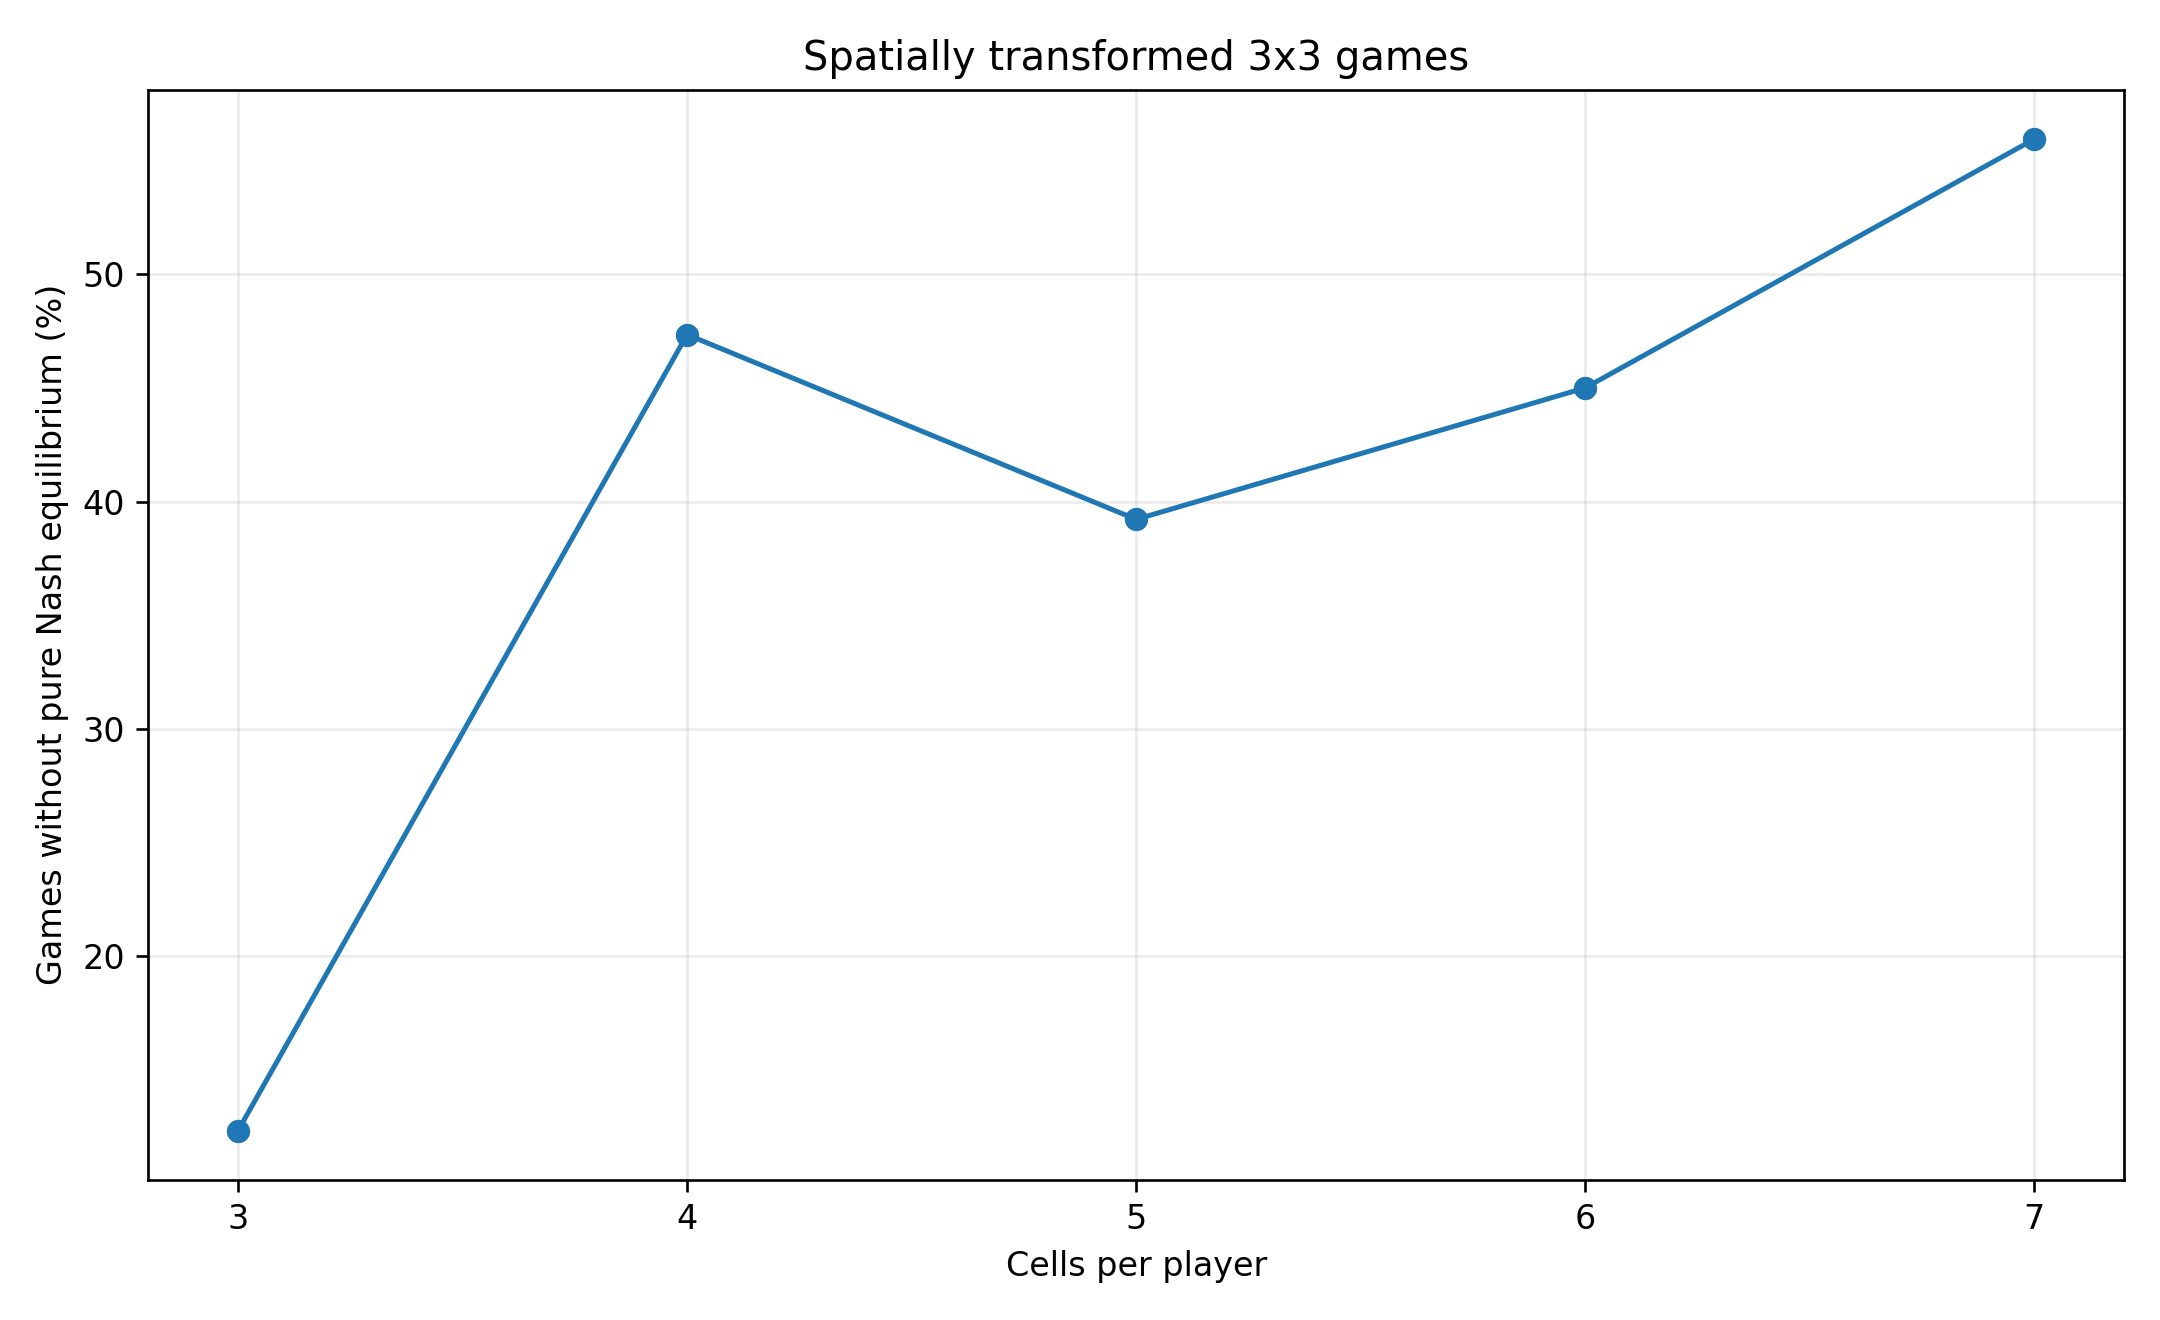
\includegraphics[width=.82\linewidth]{figures/fig04_spatial_sensitivity.png}
\caption{Absence of a pure-strategy equilibrium across the sixteen paired spatial-transform combinations per independent three-action strategy set. Transformations are dependent within each set, so the plotted proportions should not be interpreted as based on 640 independent samples per budget.}\label{fig:spatial}
\end{figure}

This result establishes sensitivity \emph{within the declared coordinate transformations and restricted strategy sets}. It does not show that a uniform translation, rotation, or other global isometry of an unrestricted automaton necessarily changes equilibrium structure.

\subsection{Strategy-Space Scaling}\label{sec:scaling_results}

Table~\ref{tab:scaling} summarizes the central scaling experiment. For each seed budget, one hundred independently sampled ten-action pools were used to build paired matrices of size $3\times3$, $5\times5$, and $10\times10$. The probability of \emph{not} finding a pure saddle point is higher for the largest than for the smallest action set in every reported budget condition, but individual nested sets may behave differently.

\begin{table}[H]
\centering
\caption{Sampled restricted games lacking a pure zero-sum equilibrium (out of 100 games at each budget and action count). The final three columns give mean mixed minimax values in live cells at Generation 10. Action sizes are nested within each independently drawn ten-action pool.}
\label{tab:scaling}
\begin{tabularx}{\linewidth}{@{}c *{6}{>{\centering\arraybackslash}X}@{}}
\toprule
\textbf{Seeds/} & \multicolumn{3}{c}{\textbf{No pure equilibrium (\%)}} & \multicolumn{3}{c}{\textbf{Mean minimax value}}\\
\cmidrule(lr){2-4}\cmidrule(lr){5-7}
\textbf{player} & $3\times3$ & $5\times5$ & $10\times10$ & $3\times3$ & $5\times5$ & $10\times10$\\
\midrule
3 & 15 & 31 & 51 & 0.985 & 1.050 & 1.288\\
4 & 36 & 74 & 96 & 2.539 & 2.747 & 3.049\\
5 & 39 & 74 & 94 & 2.284 & 2.478 & 2.612\\
6 & 42 & 72 & 94 & 3.050 & 2.829 & 3.016\\
7 & 53 & 85 & 99 & 3.229 & 3.599 & 3.749\\
\bottomrule
\end{tabularx}
\end{table}

\begin{figure}[H]
\centering
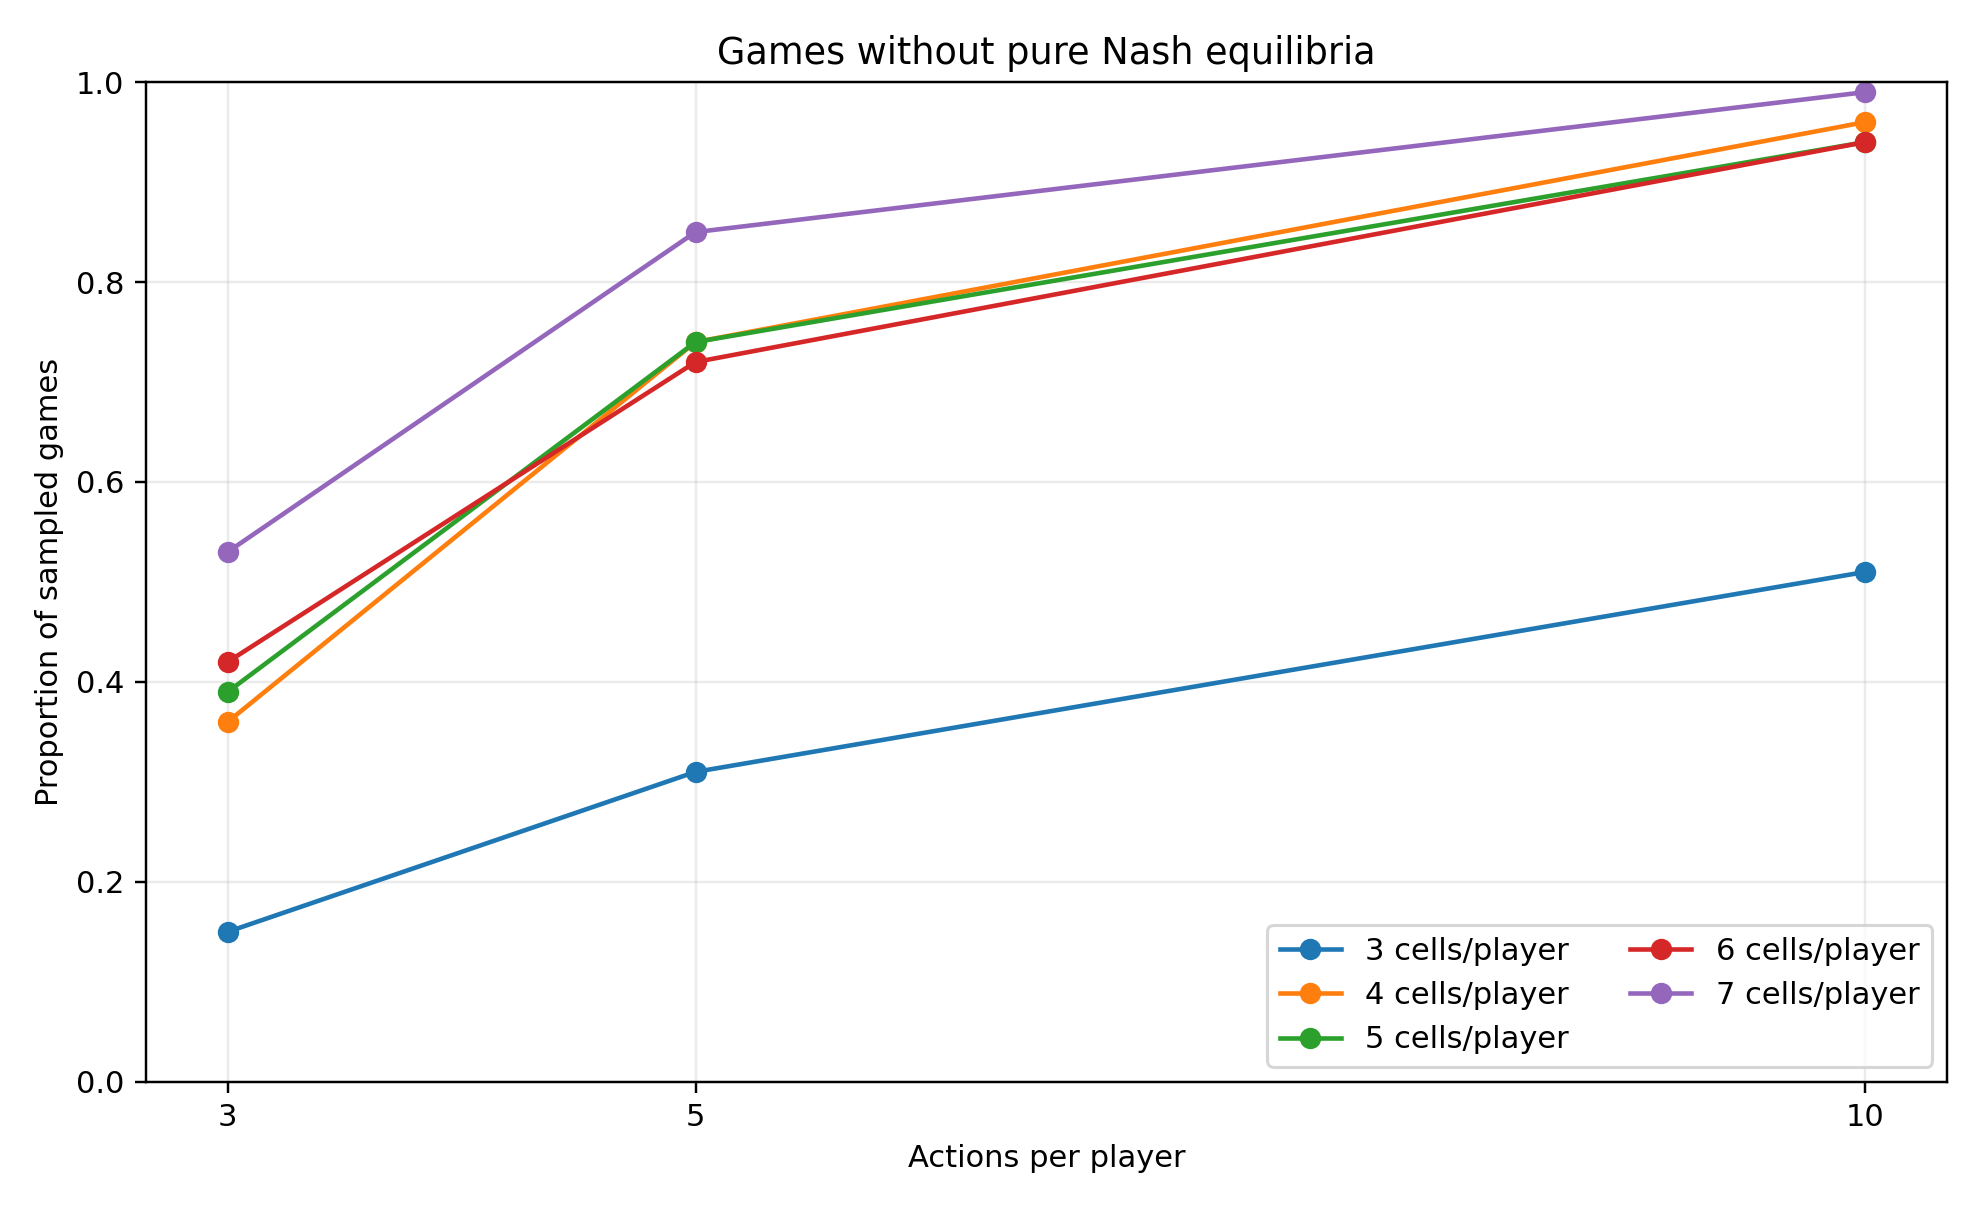
\includegraphics[width=.90\linewidth]{figures/fig03_strategy_space_scaling.png}
\caption{Observed proportions of sampled Conway-induced games without a pure saddle point for 3, 5, and 10 actions per player. All matrices use the same finite $5\times5$ domain. Comparisons across action counts are paired because each smaller matrix is a subgame of a common sampled ten-action matrix.}\label{fig:scaling}
\end{figure}

At budget three, 15\% of three-action games lacked a pure equilibrium compared with 51\% of ten-action games; at budget seven, the corresponding rates were 53\% and 99\%. At budget four, 96\% of the ten-action games lacked a pure equilibrium. The minimax game value did not obey a universal monotonic relationship with action count: for budget six, for example, the mean value was 3.050 at three actions, 2.829 at five actions, and 3.016 at ten actions. Expanding both players' available actions changes the security options of both sides, so monotonicity of the value is not implied by the minimax theorem.

These results characterize \emph{randomly sampled normal-form restrictions}, rather than a Nash equilibrium of the complete region-constrained action space or of arbitrary seeding anywhere on the board. Moreover, the rates cannot be extrapolated to larger boards without further experiments.

\subsection{Within-Matrix Payoff-Permutation Baselines}\label{sec:permutation_results}

The tie-preserving control experiment generated 200 shuffled payoff matrices for each of the 1,500 original games, yielding 300,000 permuted matrices. Across all 15 seed-budget/action-count combinations, the original Conway-derived payoff matrices exhibited lower mean rates of no-pure-equilibrium games than the corresponding shuffled controls. However, the differences were highly heterogeneous and several paired intervals included zero; thus the direction alone should not be presented as a universally significant effect.

\begin{table}[H]
\centering
\caption{Selected comparisons against tie-preserving within-matrix payoff permutations. Differences are calculated as Conway minus shuffled-control rate in percentage points (pp). Intervals are 95\% game-level paired bootstrap intervals across 100 original games per condition; the 200 controls per game are not independent experimental units.}\label{tab:permutation}
\begin{tabularx}{\linewidth}{@{}c c r r r X@{}}
\toprule
\textbf{Seeds/} & \textbf{Actions} & \textbf{Conway} & \textbf{Permuted} & \textbf{Difference} & \textbf{95\% paired interval}\\
\textbf{player} & & \textbf{(\%)} & \textbf{(\%)} & \textbf{(pp)} & \textbf{(pp)}\\
\midrule
3 & $3\times3$ & 15.0 & 26.8 & $-11.8$ & $[-18.1,-5.4]$\\
3 & $5\times5$ & 31.0 & 43.8 & $-12.8$ & $[-20.5,-5.3]$\\
3 & $10\times10$ & 51.0 & 75.1 & $-24.1$ & $[-32.6,-15.8]$\\
4 & $10\times10$ & 96.0 & 99.2 & $-3.2$ & $[-7.2,\,0.0]$\\
5 & $5\times5$ & 74.0 & 74.9 & $-0.9$ & $[-8.8,\,6.5]$\\
6 & $5\times5$ & 72.0 & 83.4 & $-11.4$ & $[-18.8,-4.2]$\\
6 & $10\times10$ & 94.0 & 99.0 & $-5.0$ & $[-10.0,-0.9]$\\
7 & $10\times10$ & 99.0 & 99.6 & $-0.6$ & $[-2.7,\,0.5]$\\
\bottomrule
\end{tabularx}
\end{table}

\begin{figure}[H]
\centering
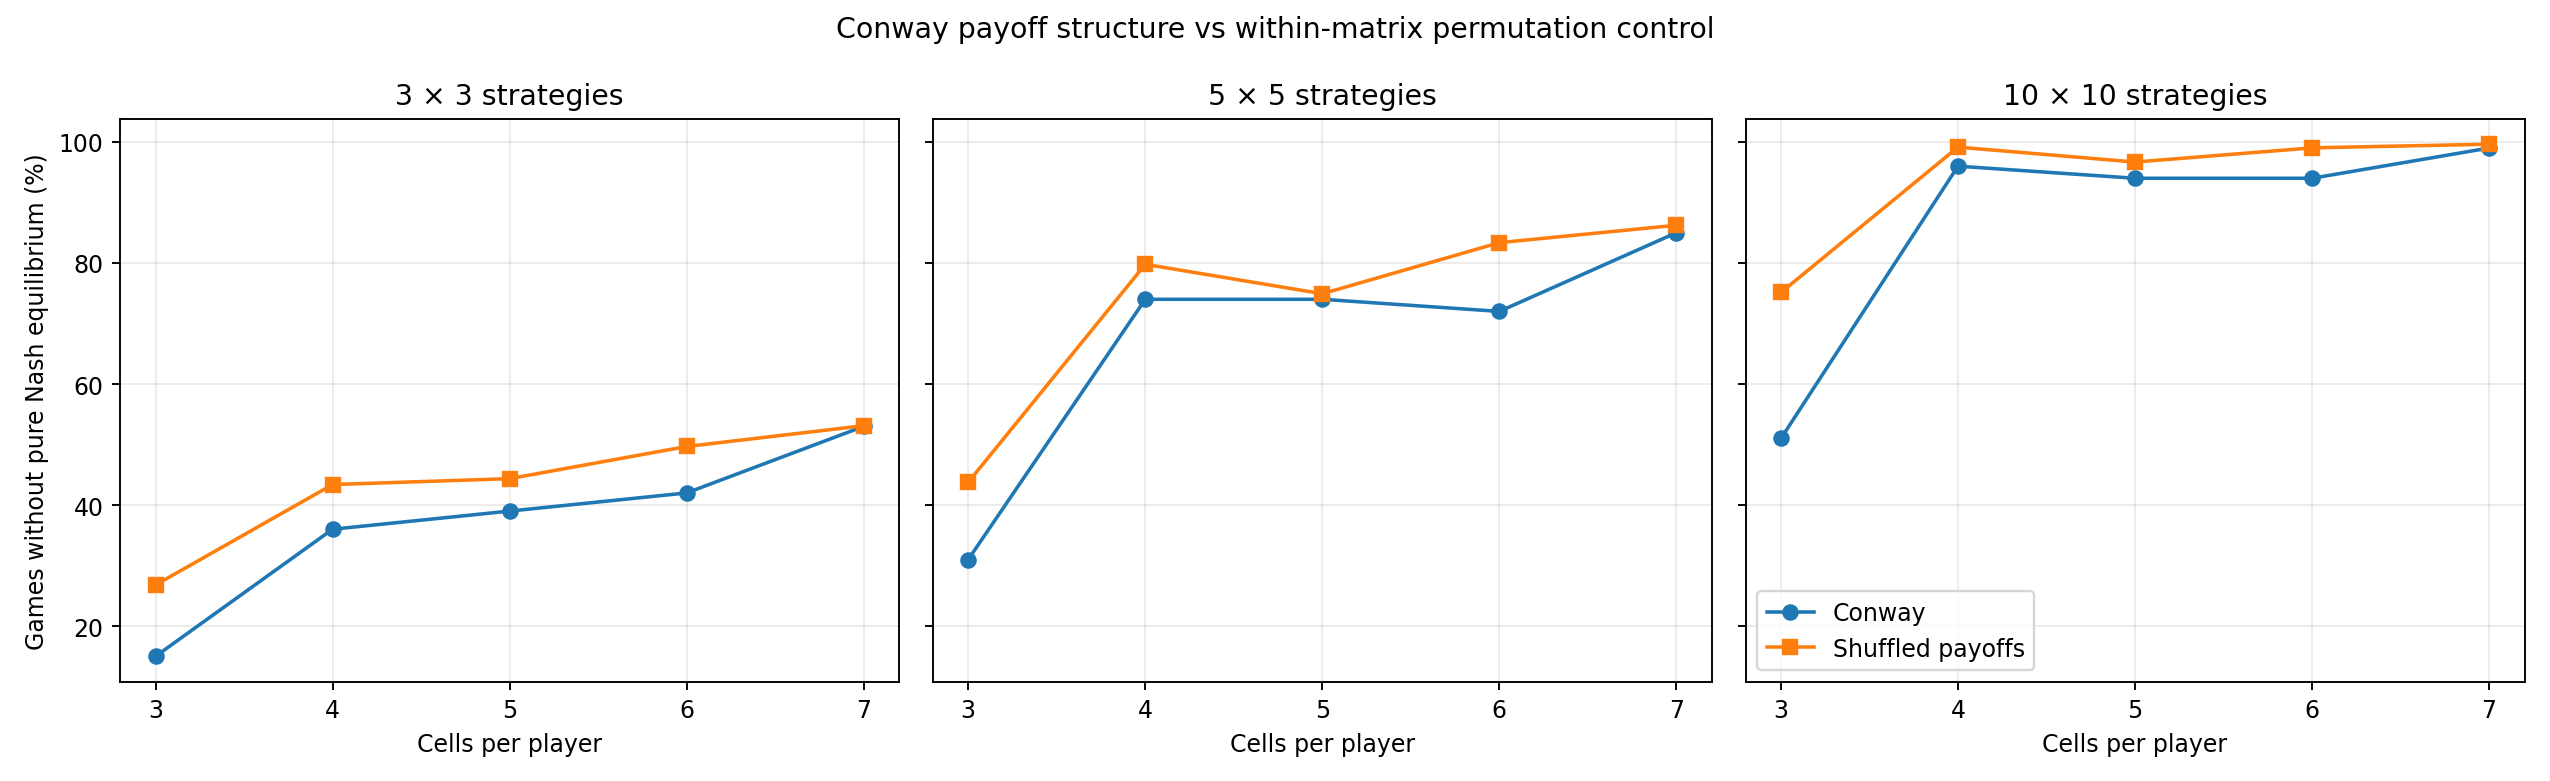
\includegraphics[width=.92\linewidth]{figures/fig05_permutation_baseline.png}
\caption{Observed proportion of original restricted Conway games lacking a pure saddle point, compared with the corresponding within-matrix permutation-control rates. Each control preserves its original matrix's exact discrete payoff multiset and ties.}\label{fig:permuted}
\end{figure}

\begin{figure}[H]
\centering
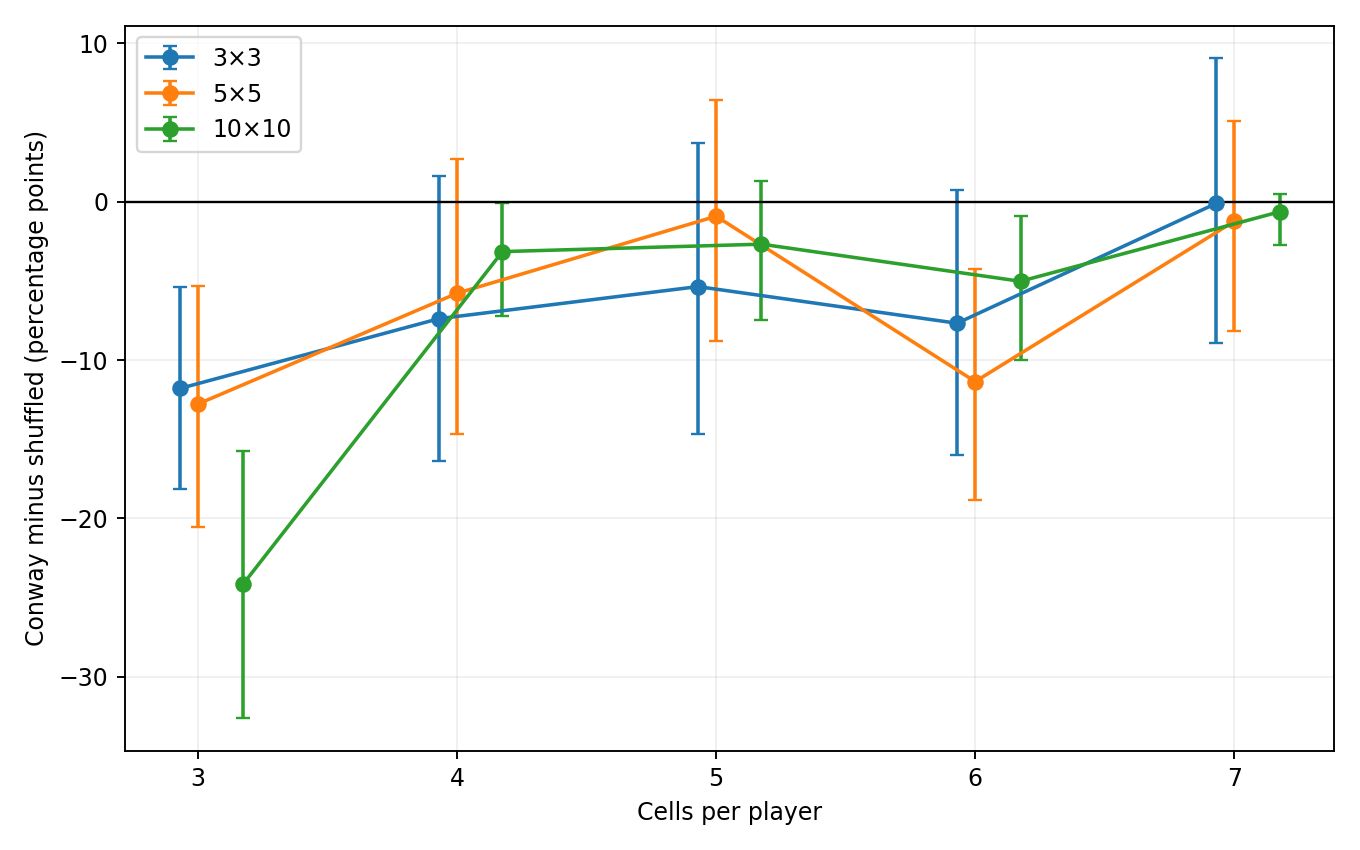
\includegraphics[width=.78\linewidth]{figures/fig06_paired_differences.png}
\caption{Paired, game-level bootstrap comparisons between observed and tie-preserving permutation-control no-pure-equilibrium rates. Intervals crossing zero represent effects not distinguished from zero by the displayed descriptive interval. Analyses involve 15 related comparisons, for which multiplicity has not been controlled.}\label{fig:paired}
\end{figure}

The most pronounced example was budget three with ten actions per player, where the observed no-pure-equilibrium rate was 51.0\%, compared with 75.13\% for the permuted controls, a difference of $-24.13$ percentage points (paired 95\% interval approximately $[-32.6,-15.8]$ pp). By contrast, at budget seven with ten actions, both observed and control matrices almost always lacked a pure saddle point (99.0\% and approximately 99.64\%, respectively), leaving little room for an informative absolute-rate difference. The results are compatible with a nonarbitrary row--column organization of the payoff matrix relative to shuffled controls, but they cannot uniquely attribute that organization to the Conway update independently of the spatial seeding restrictions.

\subsection{Cross-Platform State Agreement}\label{sec:validation_results}

All ten selected NES-observed trajectories matched the corresponding Python expectations at each of the ten recorded generations: $100/100$ entire $5\times5$ boards and $2{,}500/2{,}500$ individual cell positions. Terminal populations were therefore also identical for these selected cases. The ten cases included extinction and survival patterns, pure-equilibrium pairings, and spatial-sensitivity examples selected from the computational datasets.

\begin{figure}[H]
\centering
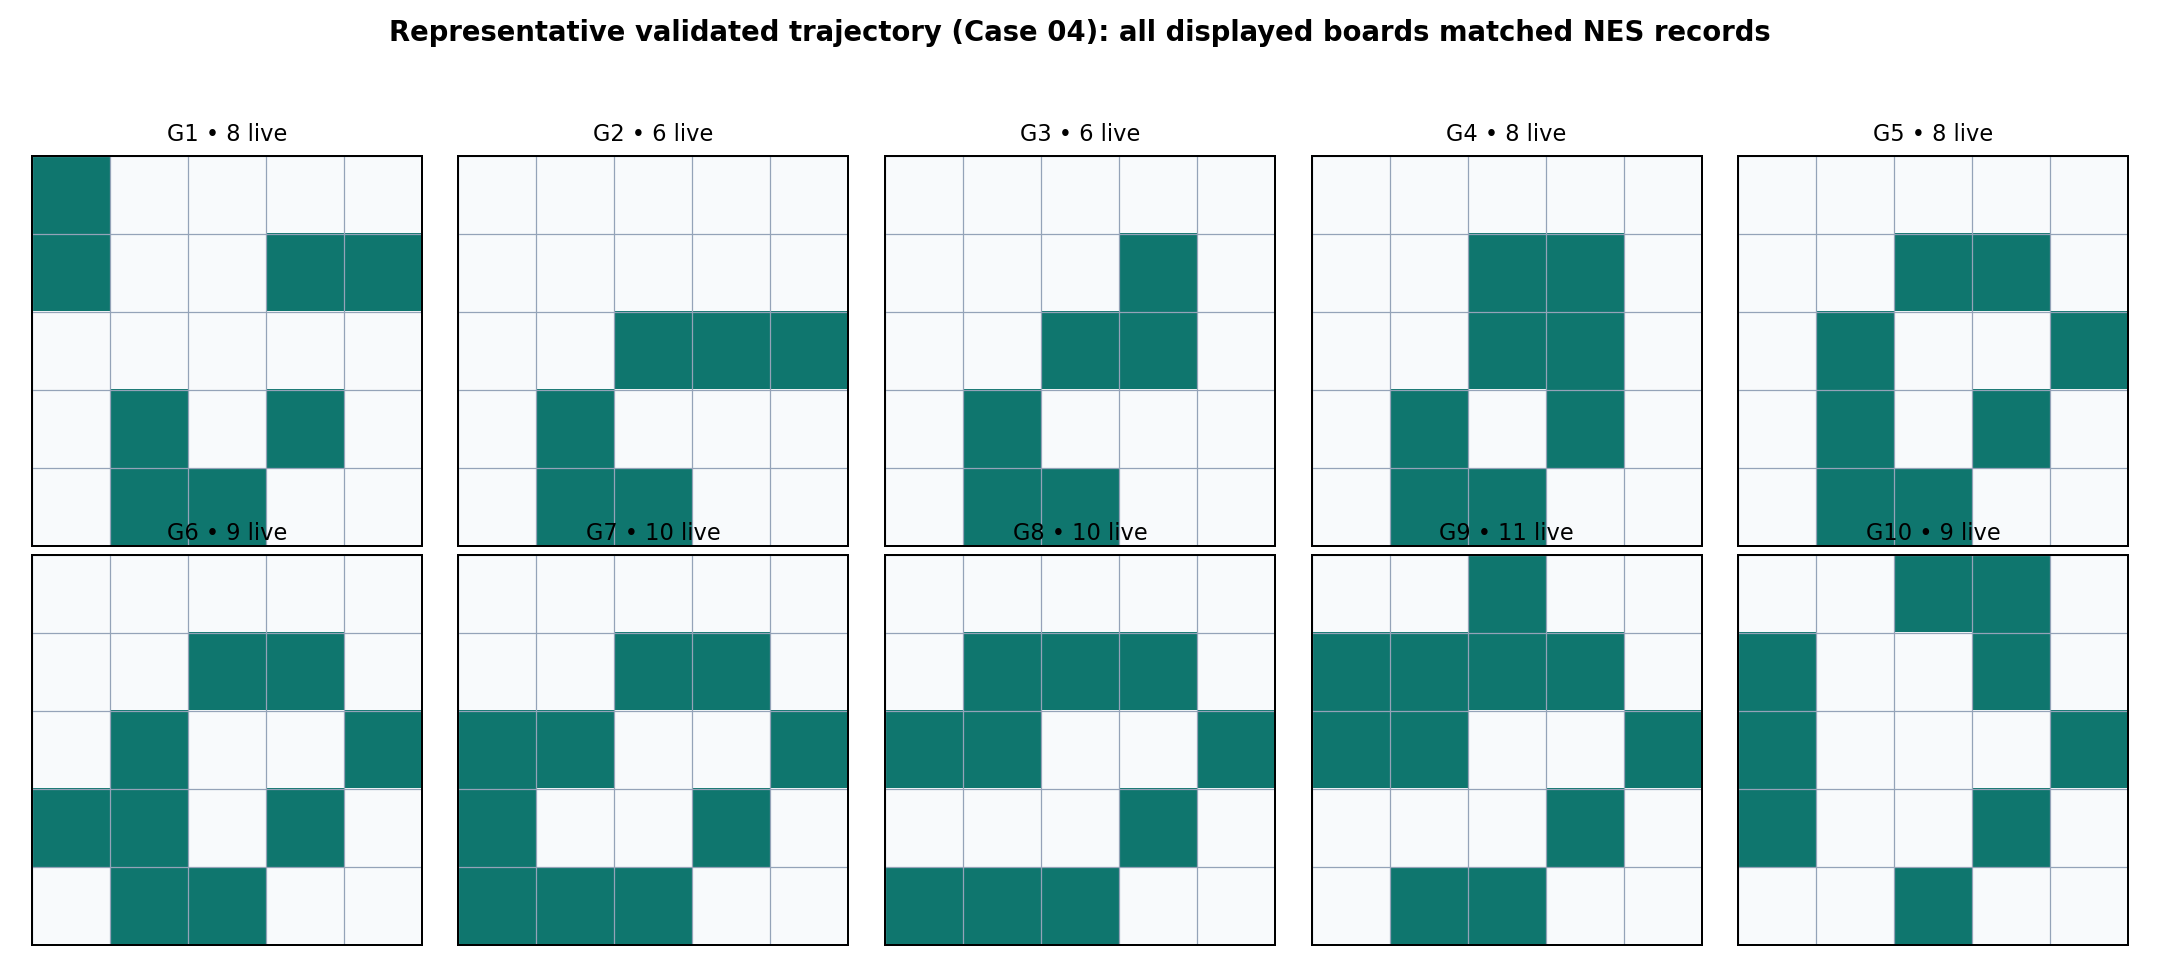
\includegraphics[width=.91\linewidth]{figures/fig07_nes_python_trajectory.png}
\caption{Illustrative Generation 1--10 trajectory for validation Case 04, reconstructed from the binary row records. All shown reference boards matched the NES observations. This is a visualization of the transcribed validation data, \emph{not} a photograph of the NES display or evidence of a two-player console implementation.}\label{fig:nesmatch}
\end{figure}

Figure~\ref{fig:nesvisual} additionally illustrates the comparison workflow using representative stable, oscillatory, boundary-sensitive, and randomly initialized configurations. For each example, the binary-board representation is displayed alongside the corresponding NES screen at Generations 1, 2, and 10. These screenshots provide qualitative visual context for the board-state comparison; they do not replace the cell-by-cell verification reported above, nor do they imply that the NES executes the two-player game-theoretic analysis.

\begin{figure}[H]
\centering
% Upload fig12_nes_python_visual_comparison.jpg into figures/.
% The conditional placeholder keeps the project compilable before upload.
\IfFileExists{figures/fig12_nes_python_visual_comparison.jpg}{%
  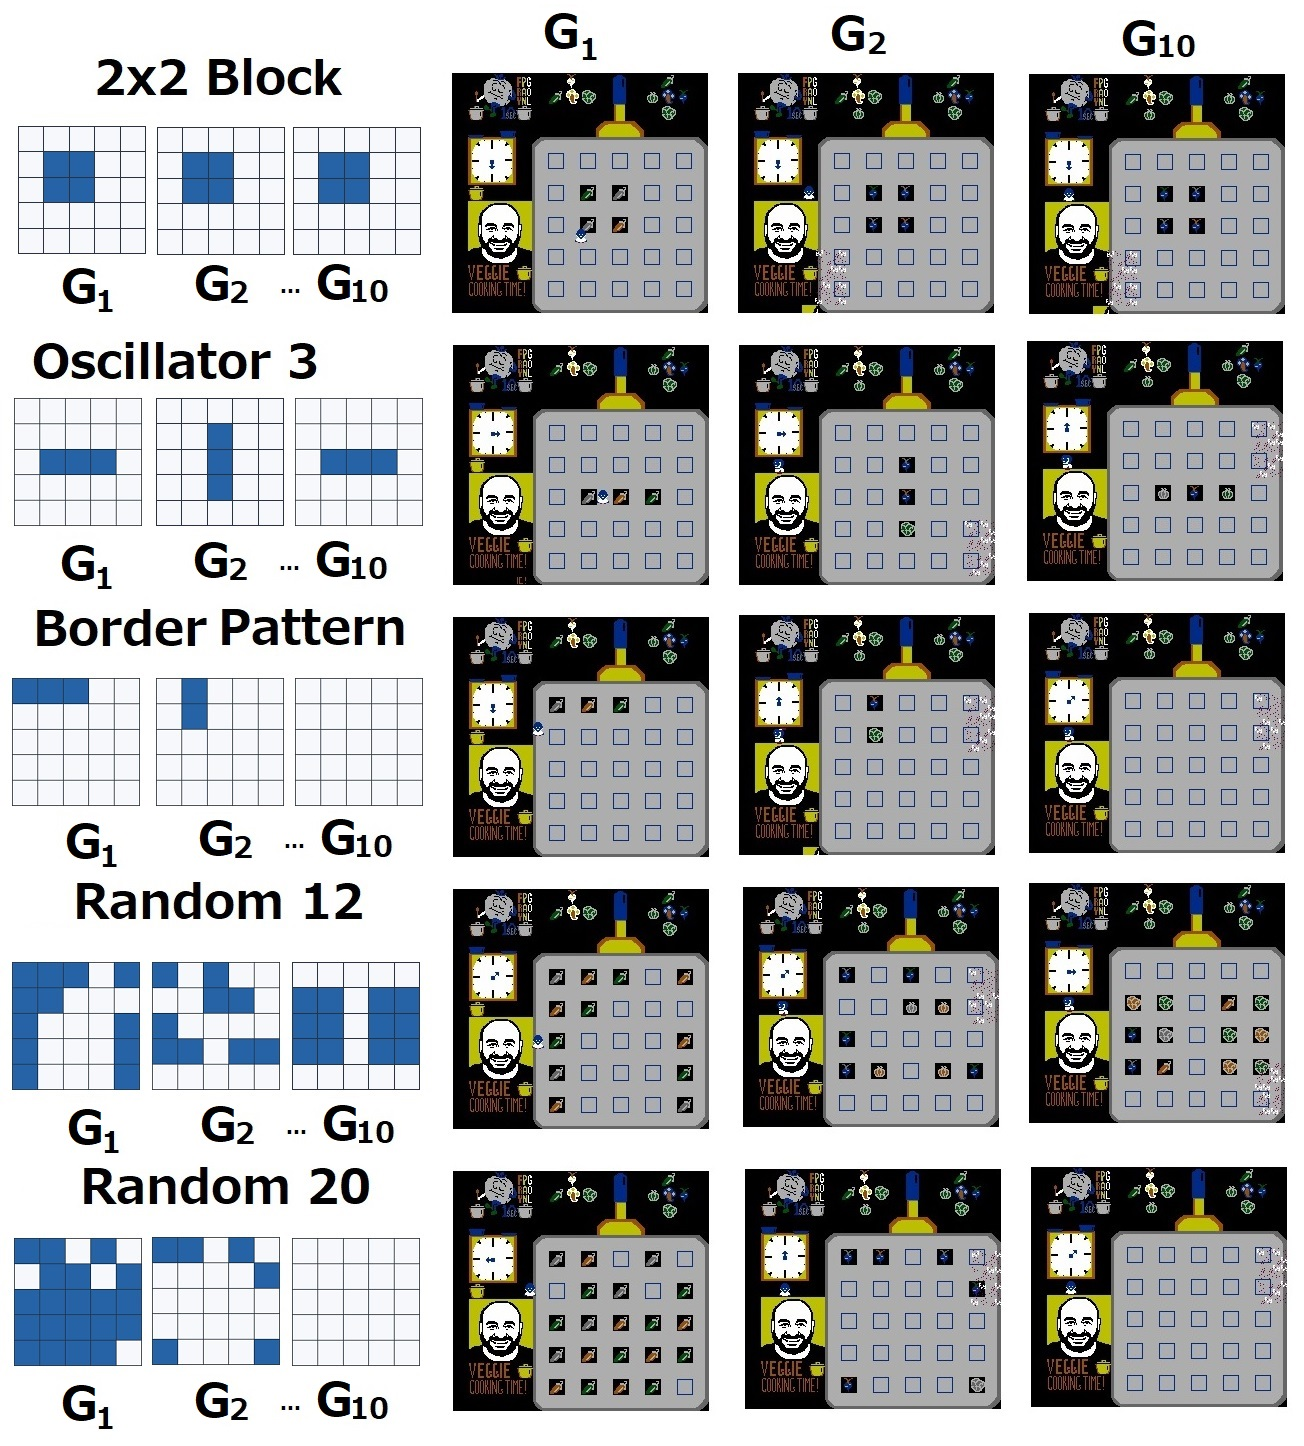
\includegraphics[width=\linewidth]{figures/fig12_nes_python_visual_comparison.jpg}%
}{%
  \fbox{\parbox[c][4cm][c]{.90\linewidth}{\centering Figure pending upload:\\ \texttt{fig12\_nes\_python\_visual\_comparison.jpg}}}%
}
\caption{Representative visual comparison of binary $5\times5$ Conway states and NES screenshots at Generations 1, 2, and 10. The examples show a stable $2\times2$ block, a three-cell period-two oscillator (blinker), a boundary-sensitive pattern, and two random initial configurations with 12 and 20 live cells. These five illustrated trajectories are examples of the cross-platform comparison workflow; the quantitative validation reported in the text comprises ten selected trajectories and 100 complete board-state comparisons.}
\label{fig:nesvisual}
\end{figure}

The agreement supports execution-level consistency between the selected GoL transitions on the NES implementation and the Python reference under the specified finite-board and generation-count convention. It does not prove correctness of the linear-programming solver on the NES, since that solver did not run on the console, nor does it constitute exhaustive testing of all region-constrained profiles.

\section{Discussion}\label{sec:discussion}

\subsection{What the Equilibrium Results Establish}

The primary result is that a familiar one-species deterministic cellular automaton can induce nontrivial finite zero-sum normal-form games when independent parties compete over the arrangement of initial live cells. The existence of pure equilibria depends on the specified action restrictions, seed budget, and relative geometry. The mixed minimax solution remains well defined in every finite case, as expected from classical game theory \citep{vonNeumann1944,nash1951}. The spatial transformation results demonstrate that the identity of a restricted strategy set matters, rather than only the total number of initially occupied sites.

Our analysis should not be interpreted as evidence of an endogenous ownership mechanism or of two competing biological populations. Unlike the competitive automata of \citet{levene2003} and the Immigration Game framework studied by \citet{turney2021}, the transition function has no information about which player supplied a live cell. Competition resides entirely in the externally defined payoffs. This distinction preserves the canonical cellular dynamics and isolates strategic decisions at initialization, but also limits the biological interpretation of the model.

A second contribution is the empirical comparison with payoff-permutation controls. Ties are central to finite-horizon, integer-valued GoL payoff matrices. Comparing these matrices directly with continuous independent random-matrix saddle-point formulas can be misleading \citep{thorp1979}. A within-matrix permutation preserves the observed discreteness and all ties. The resulting comparisons suggest structural dependencies among payoffs that are lost when row--column organization is randomized. Yet some intervals cross zero, and the randomized control does not isolate every modeling decision: the cells are drawn from disjoint spatial regions and each matrix row/column repeatedly reuses the same player's initial strategy. More discriminating future controls could preserve such dependence or replace Conway evolution with alternative deterministic dynamics while holding the spatial and sampling designs fixed.

\subsection{Interpretation of the NES Connection}

The NES implementation contributes a distinct methodological role, consistent with the distinction between platform constraints and the analytical models executed outside the console \citep{altice2015,senzio2026nes}. Its acquisition stage creates a concrete interpretation of a finite seed budget, and its placement interface makes initial conditions observable and manually configurable. Its 6502-era constraints also provide a contrasting execution environment for testing a subset of transitions. Nevertheless, no users were enrolled as strategic decision makers, the first stage was not modeled as a strategic budget-acquisition game, and the console did not compute normal-form equilibria. These statements prevent an unwarranted inference from a playable artificial-life system to validated human game-theoretic behavior.

The exploratory initialization data also clarify the motivation for the formal model: at a fixed total initial density of 12, manually selected patterns displayed substantial differences in finite-horizon persistence. Nevertheless, those descriptive persistence measures are not directly comparable to the zero-sum terminal-population payoff, and manual pattern families should not be interpreted as equilibrium strategies. The earlier random--manual comparison involved unequal and nonrandomly selected configuration sets; it is therefore not a causal test of initialization mode.

This article is deliberately centered on formal strategic interaction rather than on the platform implementation or a broader descriptive density survey. The connection to interactive seed initialization serves to define a feasible methodological context; the distinctive analytical object is the terminal-population payoff matrix and its equilibrium structure. Future work should separate the descriptive study of emergence, interactive experiments with human users, and competitive mathematical decision models.

\subsection{Limitations and Next Steps}

There are five key limitations. First, the $5\times5$ board and nine-update horizon are selected to correspond to the existing implementation; conclusions need not transfer to larger or asymptotic systems. Second, all equilibria are equilibria \emph{of sampled action subsets}, not the fully region-constrained game, and not unrestricted all-board seeding. Third, the asymmetric top/bottom domain and initially empty middle row may introduce boundary-related effects; no claim of spatial neutrality is made. Fourth, the permutation controls preserve payoff frequencies and ties but not shared-strategy dependence, and multiple exploratory conditions are examined without a prespecified familywise adjustment. Fifth, the ten NES cases are selected validations and not representative statistical samples of the whole configuration space.

Future work can perform exact enumeration of the full region-constrained action spaces where computationally feasible; compare alternative payoff objectives (including persistence and ownership-preserving species models); introduce matched controls that separately manipulate the cellular update and seeding geometry; and investigate larger boards and longer horizons. A separate future study could recruit participants to compare manual seed placement with random baselines and theoretically optimal mixed play, including learning and behavior across repeated trials. Such a human-participant experiment is not necessary to support the current purely computational claims and is outside the present budget and schedule.

\section{Conclusions}\label{sec:conclusion}

We developed a finite two-player zero-sum framework in which separate, fixed-cardinality initial seed choices induce a payoff matrix from an unchanged Conway B3/S23 automaton. Empirical analysis of 1,500 sampled nested action-set games shows that pure-equilibrium availability is sensitive to the number and arrangement of the strategies under consideration. A related spatial study confirms substantial variation under prescribed seed-coordinate transformations. Tie-preserving payoff-permutation controls provide evidence that strategic row--column organization can differ from randomized arrangements, particularly for low-budget, larger-action conditions, while also underscoring the limits of attributing this effect to Conway dynamics alone. Finally, ten selected trajectories agreed cell-for-cell with NES observations, linking the analytical reference to the existing constrained interactive implementation. The conclusions are restricted to the reported normal-form sampling protocol and finite observation horizon; they make no claim about strategic human behavior or globally optimal unrestricted seed placements.

\vspace{6pt}
\authorcontributions{\textbf{Preliminary placeholder:} Final CRediT roles (conceptualization, methodology, software, validation, formal analysis, visualization, writing, supervision, and project administration) are to be confirmed and approved by Bruno Senzio-Savino, Faramarz Alsharif, Aleksandar Shurbevski, and Mahdi Khosravy before submission. No contributions have been assigned to individual coauthors without their confirmation.}

\institutionalreview{Not applicable. This article reports computational simulations and comparison of implemented automaton states; no human participants or animals were studied.}
\informedconsent{Not applicable. No human-participant study was conducted.}
\dataavailability{Source code, machine-readable summary tables, and the NES--Python binary observation table accompany this preliminary draft. The exploratory density and manual--random summary statistics require verification against the original run-level data before submission; original image provenance should also be confirmed. A permanent publicly accessible archive or DOI is to be supplied before submission; no repository URL is claimed as finalized here. The NES ROM and any distribution permissions should be reviewed separately before public release.}
\acknowledgments{\textbf{Generative AI disclosure (draft):} During the preparation of this manuscript, the authors used OpenAI ChatGPT to assist with the organization and drafting of scientific text, LaTeX preparation, and visual presentation of existing data. All mathematical definitions, reported results, reference details, scripts, and figures must be reviewed and approved by the authors, who retain full responsibility for the article. The wording and specific tools used should be updated to reflect the final submission process.}
\conflictsofinterest{\textbf{To be confirmed with all authors.} No declaration has been inferred from the supplied affiliations.}

% External BibTeX bibliography: use the official MDPI class bibliography style.
% Do not also paste the example thebibliography block from the MDPI template.
\reftitle{References}
\bibliography{references}
\PublishersNote{}
\end{document}